\documentclass[onehalfspacing]{article}

\usepackage{amsmath,amssymb,amsthm}
\usepackage{ wasysym }
\usepackage{ stmaryrd }
\usepackage{ mathpartir }
\usepackage{xcolor}
\usepackage{bussproofs}
\usepackage[left=2.00cm, right=2.00cm, top=2.00cm,bottom=2.0cm]{geometry}
\usepackage{pdflscape}
\usepackage{xspace}
\usepackage{todonotes}
\usepackage{stackengine}
\usepackage{tikz}
\usepackage{tikz-qtree}


\setlength\parindent{0pt}

\theoremstyle{definition}
\newtheorem{theorem}{Theorem}[section]
\theoremstyle{definition}
\newtheorem{corollary}[theorem]{Corollary}
\theoremstyle{definition}
\newtheorem{lemma}[theorem]{Lemma}
\theoremstyle{definition}
\newtheorem{proposition}[theorem]{Proposition}
\theoremstyle{definition}
\newtheorem{definition}[theorem]{Definition}
\theoremstyle{definition}
\newtheorem{example}[theorem]{Example}

\newcommand{\llb}{\llbracket}
\newcommand{\rrb}{\rrbracket}
\newcommand{\blue}[1]{{\color{blue}#1}}
\newcommand{\var}{\text{var}}
\newcommand{\Gc}{\textbf{Gc}\xspace}
\newcommand{\Gi}{\textbf{Gi}\xspace}
\newcommand{\Res}{\textbf{Res}\xspace}
\newcommand{\I}{\mathcal{I}}

\author{Alexander Pluska}
\title{Proofs as Programs in Classical Logic\\Notes}

\begin{document}

\maketitle

\section{Plan}

Goal:
\begin{itemize}
	\item Extract program from resolution proofs of $\forall\exists$-sentences over inductive datatypes.
\end{itemize}

\noindent Steps:

\begin{itemize}
	\item Give extensions of G\"odel's System \textbf{T} and HAS + EM$_1$ + SK$_1$ to arbitrary inductive datatypes (possibly GADTs) and prove (or rather check) properties, i.e. strong normalization, cut-elimination, uniqueness of normal forms.
	\item Adapt the results of~\cite{aschieri2014interactive} to exhibit realizers in $\mathcal{F} + \Phi$ for cut-free proofs in the extended version of HAS + EM$_1$ + SK$_1$ of formulas $\forall x\exists y Pxy$ where $P$ is a predicate in the extended version of \textbf{T}.
	\item Adapt the iterative learning from~\cite{aschieri2014interactive} to extract $\lambda$-terms from realizers.
	\item Give a proof translation from resolution proofs to cut-free sequent calculus proofs (already done?).
\end{itemize}

\noindent Questions:
\begin{itemize}
	\item When does the translated proof require more than EM$_1$?
	\item Using the methods in~\cite{aschieri2014interactive} the extracted term will be in simple $\lambda$-calculus. Is is possible to obtain a term in $\mathcal{F}$? (Talk with Federico Aschieri)
	\item Can the predicates be defined in $\mathcal{F}$ instead of $\mathcal{T}$? (probably yes)
	\item What happens if we add non-inductive theories?
	
\end{itemize}

\pagebreak

\pagebreak

To exdefinition our approach let us first recall how resolution works and why it is effective for classical logic. In a nutshell the principle of resolution works as follows: From a set of formulas $A, B, C\dots$ obtain a set of sequents $A'_1\dots  A'_n\vdash A_1\dots A_n$, $B'_1\dots B'_n\vdash B_1\dots B_n$, $C'_1\dots C'_n\vdash C_1\dots C_n$ in which all occurring formulas are somehow simple. Then iteratively apply the resolution rule (and some other rules, but this is the crucial one), which is an analogon to cut, i.e.
\begin{center}
	\AxiomC{$A, \Gamma\vdash \Delta$}
	\AxiomC{$\Gamma'\vdash A', \Delta'$}
	\BinaryInfC{$(\Gamma\cup \Gamma')\theta\vdash (\Delta\cup\Delta')\theta$}
	\DisplayProof
\end{center}
where $\theta$ is the mgu of $A$ and $A'$, and by process of saturation (attempt to) obtain the empty Sequent.

Now for classical logic we can simply interpret $A'_1,\dots  A'_n\vdash A_1,\dots, A_n$ as $\neg A'_1\vee\dots\vee\neg A'_n\vee A_1\vee\dots\vee A_n$. Furthermore we can normalize every formula such that each of the $A'_i, A_i$ is atomic. The resolution calculus is then immediately refutationally complete, i.e. if $A, B, C\dots $ are inconsistent there exists a successful resolution, giving a refutation of $A\wedge B\wedge C\dots$, which is classically equivalent to a proof of $B\wedge C\dots\rightarrow\neg A$. I.e. if we want to prove $B\wedge C\dots\rightarrow A$ we can simply perform resolution on $\neg A\wedge B\wedge C\dots$

Now there are a number of hurdles in applying this strategy to intuitionistic logic, or to extract intuitionistic proof from classical resolution proofs. First and foremost is the non-existence of normal forms. In particular with the (intuitionally speaking) strict interpretation of $A'_1,\dots  A'_n\vdash A_1,\dots, A_n$ as $\neg A'_1\vee\dots\vee\neg A'_n\vee A_1\vee\dots\vee A_n$ we can hardly translate any formulas into such a form where the $A_i$ are atomic, or even literals. This can be remedied of course by interpreting $A'_1,\dots  A'_n\vdash A_1,\dots, A_n$ as $\neg(A'_1\wedge\dots\wedge A'_n\wedge(\neg A_1\vee\dots\vee \neg A_n))$, i.e. a double negation translation. But this brings us to the second problem: Even if our calculus is refutationally complete a refutation of $\neg A\wedge B\wedge C\dots$ does not give us a proof of $B\wedge C\dots\to A$ but rather $B\wedge C\dots\to \neg\neg A$. This problem is especially pronounced in the second interpretation of $\vdash$ where we are not even using $A$ but $\neg \neg A$.

Now there are a few saving graces: First of all, if $A$ is decidable, i.e. $\neg\neg A\to A$, we immediately obtain a proof of $A$. Furthermore we may attempt Friedman Translation~\cite{Friedman_1978} of our proof and indeed~\cite{Berger_2002} gives us some quite liberal criteria when this is possible in principle, e.g. when $B, C\dots$ are theorems of PA and $A$ is a $\Pi_0^2$ formula. And indeed interpreting $A'_1,\dots  A'_n\vdash A_1,\dots, A_n$ as $A'_1\to\dots\to A'_n\to A_1\vee\dots\vee A_n$, we are able to obtain an intuitionistic proof if their conditions are met and the input formulas can be transformed to such normal forms.

\section{Extracting constructive content from resolution proofs}
\subsection{The superposition calculus}
First let us define the calculus from which we wish to extract programs. It will comprise a core set of rules used in the vampire theorem prover taken from~\cite{Kov_cs_2013}. Note that we pay special attention to the usually neglected (and highly non-constructive) part of CNF transformation and Skolemization. Also note that we neglect the simplification ordering which is necessary to formulate a strategy for proof search but not for our proof transformation.

\noindent\textbf{Resolution.}
\begin{center}
\AxiomC{$A\vee B$}
\AxiomC{$\neg A'\vee C$}
\BinaryInfC{$(B\vee C)\theta$}
\DisplayProof
\end{center}
where $\theta$ is an mgu of $A$ and $A'$.

\noindent\textbf{Factoring.}
\begin{center}
	\AxiomC{$A\vee A'\vee B$}
	\UnaryInfC{$(A\vee B)\theta$}
	\DisplayProof
\end{center}
where $\theta$ is an mgu of $A$ and $A'$.

\noindent\textbf{Superposition.}
\begin{center}
	\AxiomC{$l=r\vee B$}
	\AxiomC{$L[s]\vee C$}
	\BinaryInfC{$(L[r]\vee B\vee C)\theta$}
	\DisplayProof
	\AxiomC{$l=r\vee B$}
	\AxiomC{$t[s] = t'\vee C$}
	\BinaryInfC{$(t[r] = t'\vee B\vee C)\theta$}
	\DisplayProof
	\AxiomC{$l=r\vee B$}
	\AxiomC{$t[s]\neq t'\vee C$}
	\BinaryInfC{$(t[r]\neq t'\vee B\vee C)\theta$}
	\DisplayProof
\end{center}
where $\theta$ is an mgu of $l$ and $s$, $s$ is not a variable, $L[s]$ is not an equality literal.

\noindent\textbf{Equality Resolution.}
\begin{center}
	\AxiomC{$s\neq t\vee C$}
	\UnaryInfC{$C\theta$}
	\DisplayProof
\end{center}
where $\theta$ is an mgu of $s$ and $t$.

\noindent\textbf{Equality Factoring.}
\begin{center}
	\AxiomC{$s=t\vee s'=t'\vee C$}
	\UnaryInfC{$(s=t\vee t\neq t'\vee C)\theta$}
	\DisplayProof
\end{center}
where $\theta$ is an mgu of $s$ and $s'$.

First let us look at an example of the transformation we going to do. We shall look at a proof of $\forall x\exists y: f(y) = g(x)$ from $\forall x: f(x) = g(h(x))$ and $\forall x: h(h'(x)) = x$. The program we extract hopefully is $h'$.

\begin{align}
	[\text{axiom}]&&\forall x: f(x) = g(h(x))\\
	[\text{cnf 1}]&&f(x_0) = g(h(x_0))\\
	[\text{axiom}]&&\forall x: h(h'(x)) = x\\
	[\text{cnf 3}]&&h(h'(x_0)) = x_0\\
	[\text{negated conjecture}]&&\neg\forall x\exists y: f(y) = g(x)\\
	[\text{ennf 5}]&&\exists x\forall y: f(y)\neq g(x)\\
	[\text{choice axiom}]&&\exists x\forall y: f(y)\neq g(x)\rightarrow \forall x : f(x) \neq g(s_0)\\
	[\text{skolemization 6, 7}]&&\forall x: f(x)\neq g(s_0)\\
	[\text{cnf 8}]&&f(x_1)\neq g(s_0)\\
	[\text{superposition 9, 2}]&\{\}&g(s_0)\neq g(h(x_0))\\
	[\text{superposition 10, 4}]&\{x_0\mapsto h'(x_0)\}&g(x_0)\neq g(s_0)\\
	[\text{equality resolution 11}]&&\bot
\end{align}

We first use the well known trick of adding the original conjecture to the negated one from~\cite{Luckham_1971} to transform this into a classical proof of $\forall x\exists y: f(x) = g(y)$ rather than a refutation of its negation:
\setcounter{equation}{0}
\begin{align}
	[\text{axiom}]&&\forall x: f(x) = g(h(x))\\
	[\text{cnf 1}]&&f(x_0) = g(h(x_0))\\
	[\text{axiom}]&&\forall x: h(h'(x)) = x\\
	[\text{cnf 3}]&&h(h'(x_0)) = x_0\\
	[\text{\color{red}{tautology}}]&&\forall x\exists y: f(y) = g(x)\vee\neg\forall x\exists y: f(y) = g(x)\\
	[\text{ennf 5}]&&\forall x\exists y: f(y) = g(x)\vee\exists x\forall y: f(y)\neq g(x)\\
	[\text{choice axiom}]&&\exists x\forall y: f(y)\neq g(x)\rightarrow \forall x : f(x) \neq g(s_0)\\
	[\text{choice axiom}]&&\forall x(\exists y: f(y)= g(x)\rightarrow f(s_1(x)) = g(x))\\
	[\text{skolemization 6, 7}]&&\forall x\exists y: f(y) = g(x)\vee\forall x: f(x)\neq g(s_0)\\
	[\text{skolemization 9, 8}]&&\forall x: f(s_1(x)) = g(x)\vee\forall x: f(x)\neq g(s_0)\\
	[\text{cnf 8}]&&f(s_1(x_1)) = g(x_1)\vee f(x_0)\neq g(s_0)\\
	[\text{superposition 11, 2}]&\{\}&f(s_1(x_1)) = g(x_1)\vee g(s_0)\neq g(h(x_0))\\
	[\text{superposition 12, 4}]&\{x_0\mapsto h'(x_0)\}&f(s_1(x_1)) = g(x_1)\vee g(x_0)\neq g(s_0)\\
	[\text{equality resolution 13}]&\{x_0\to s_0\}&f(s_1(x_1)) = g(x_1)
\end{align}

Next we eliminate free variables by propagating substitutions:

\setcounter{equation}{0}
\begin{align}
	[\text{axiom}]&&\forall x: f(x) = g(h(x))\\
	[\text{cnf 1}]&&f(h'(x_0)) = g(h(h'(x_0)))\\
	[\text{axiom}]&&\forall x: h(h'(x)) = x\\
	[\text{cnf 3}]&&h(h'(x_0)) = x_0\\
	[\text{tautology}]&&\forall x\exists y: f(y) = g(x)\vee\neg\forall x\exists y: f(y) = g(x)\\
	[\text{ennf 5}]&&\forall x\exists y: f(y) = g(x)\vee\exists x\forall y: f(y)\neq g(x)\\
	[\text{choice axiom}]&&\exists x\forall y: f(y)\neq g(x)\rightarrow \forall x : f(x) \neq g(s_0)\\
	[\text{choice axiom}]&&\forall x(\exists y: f(y)= g(x)\rightarrow f(s_1(x)) = g(x))\\
	[\text{skolemization 6, 7}]&&\forall x\exists y: f(y) = g(x)\vee\forall x: f(x)\neq g(s_0)\\
	[\text{skolemization 9, 8}]&&\forall x: f(s_1(x)) = g(x)\vee\forall x: f(x)\neq g(s_0)\\
	[\text{cnf 8}]&&f(s_1(x_1)) = g(x_1)\vee f(h'(x_0))\neq g(s_0)\\
	[\text{superposition 11, 2}]&\{\}&f(s_1(x_1)) = g(x_1)\vee g(s_0)\neq g(h(h'(x_0)))\\
	[\text{superposition 12, 4}]&\{\}&f(s_1(x_1)) = g(x_1)\vee g(x_0)\neq g(s_0)\\
	[\text{equality resolution 13}]&\{x_0\to s_0\}&f(s_1(x_1)) = g(x_1)
\end{align}


\setcounter{equation}{0}
\begin{align}
	[\text{axiom}]&&\forall x: f(x) = g(h(x))\\
	[\text{cnf 1}]&&f(h'(s_0)) = g(h(h'(s_0)))\\
	[\text{axiom}]&&\forall x: h(h'(x)) = x\\
	[\text{cnf 3}]&&h(h'(s_0)) = s_0\\
	[\text{tautology}]&&\forall x\exists y: f(y) = g(x)\vee\neg\forall x\exists y: f(y) = g(x)\\
	[\text{ennf 5}]&&\forall x\exists y: f(y) = g(x)\vee\exists x\forall y: f(y)\neq g(x)\\
	[\text{choice axiom}]&&\exists x\forall y: f(y)\neq g(x)\rightarrow \forall x : f(x) \neq g(s_0)\\
	[\text{choice axiom}]&&\forall x(\exists y: f(y)= g(x)\rightarrow f(s_1(x)) = g(x))\\
	[\text{skolemization 6, 7}]&&\forall x\exists y: f(y) = g(x)\vee\forall x: f(x)\neq g(s_0)\\
	[\text{skolemization 9, 8}]&&\forall x: f(s_1(x)) = g(x)\vee\forall x: f(x)\neq g(s_0)\\
	[\text{cnf 8}]&&f(s_1(x_1)) = g(x_1)\vee f(h'(s_0))\neq g(s_0)\\
	[\text{superposition 11, 2}]&\{\}&f(s_1(x_1)) = g(x_1)\vee g(s_0)\neq g(h(h'(s_0)))\\
	[\text{superposition 12, 4}]&\{\}&f(s_1(x_1)) = g(x_1)\vee g(s_0)\neq g(s_0)\\
	[\text{equality resolution 13}]&\{\}&f(s_1(x_1)) = g(x_1)
\end{align}

Next we remove all the skolem constants in the conjecture-tautology by unification, propagate this change, and finally reinterpet superposition as composition to yield a valid intuitionistic proof:

\setcounter{equation}{0}
\begin{align}
	[\text{axiom}]&&\forall x: f(x) = g(h(x))\\
	[\text{instantiation 1}]&&f(h'(x_1)) = g(h(h'(x_1)))\\
	[\text{axiom}]&&\forall x: h(h'(x)) = x\\
	[\text{instantiation 3}]&&h(h'(x_1)) = x_1\\
	[\text{tautology}]&&f(h'(x_1)) = g(x_1)\Rightarrow f(h'(x_1)) = g(x_1)\\
	[\text{equality 5, 2}]&\{\}&g(x_1)= g(h(h'(x_1)))\Rightarrow f(h'(x_1)) = g(x_1)\\
	[\text{equality 6, 4}]&\{\}&g(x_1)= g(x_1)\Rightarrow f(h'(x_1)) = g(x_1)\\
	[\text{equality 13}]&\{\}&f(h'(x_1)) = g(x_1)
\end{align}

Let us look at a second example: Consider the sentences $\forall x : p(x_0, f(x_0))$, $\forall x_0, x_1: (p(x_0, x_1)\Rightarrow q(x_0, g(x_1))$, $\forall x_0, x_1: (q(x_0, x_1)\Rightarrow r(x_0, h(x_1)))$. We take a look at a proof of $\forall x_0\exists x_1: r(x_0, x_1)$ which hopefully gives us $h\circ g\circ f$. First consider the output of vampire

\setcounter{equation}{0}
\begin{align}
	[\text{axiom}] && \forall x_0: p(x_0,f(x_0))\\
	[\text{axiom}] && \forall x_0, x_1 : (p(x_0,x_1) \Rightarrow q(x_0,g(x_1)))\\
	[\text{axiom}] && \forall x_0, x_1 : (q(x_0,x_1) \Rightarrow r(x_0,h(x_1)))\\
	[\text{negated conjecture}] &&\neg\forall  x_0 : \exists x_1 : r(x_0,x_1)\\
	[\text{ennf transformation 2}] && \forall x_0, x_1 : (q(x_0,g(x_1)) \vee \neg p(x_0,x_1)) \\
	[\text{ennf transformation 3}] &&\forall x_0, x_1 : (r(x_0,h(x_1)) \vee \neg q(x_0, x_1)) \\
	[\text{ennf transformation 4}] && \exists x_0 \forall x_1 : \neg r(x_0, x_1)\\
	[\text{choice axiom}] && \exists x_0 \forall x_1 : \neg r(x_0, x_1) \Rightarrow \forall x_1 : \neg r(s_0,x_1)\\
	[\text{skolemisation 7,8}] && \forall x_1 : \neg r(s_0, x_1)\\
	[\text{cnf transformation 1}] && p(x_0,f(x_0))\\
	[\text{cnf transformation 5}] && q(x_1,g(x_2)) \vee \neg p(x_1, x_2)\\
	[\text{cnf transformation 6}] && r(x_3,h(x_4)) \vee \neg q(x_3, x_4)\\
	[\text{cnf transformation 9}] &&. \neg r(s_0,x_5)\\
	[\text{resolution 12, 13}] &\{x_3\mapsto s_0, x_5\mapsto h(x_4)\}& \neg q(s_0,x_4)\\
	[\text{resolution 14, 11}] &\{x_1\mapsto s_0, x_4\mapsto g(x_2)\}&\neg p(s_0,x_2)\\
	[\text{resolution 15, 10}] &\{x_0\mapsto s_0, x_2\mapsto f(s_0)\}& \bot
\end{align}

Again replace negated conjecture by tautology

\setcounter{equation}{0}
\begin{align}
	[\text{axiom}] && \forall x_0: p(x_0,f(x_0))\\
	[\text{axiom}] && \forall x_0, x_1 : (p(x_0,x_1) \Rightarrow q(x_0,g(x_1)))\\
	[\text{axiom}] && \forall x_0, x_1 : (q(x_0,x_1) \Rightarrow r(x_0,h(x_1)))\\
	[\text{tautology}] &&\forall  x_0 \exists x_1 : r(x_0,x_1)\vee \neg\forall  x_0 \exists x_1 : r(x_0,x_1)\\
	[\text{ennf transformation 2}] && \forall x_0, x_1 : (q(x_0,g(x_1)) \vee \neg p(x_0,x_1)) \\
	[\text{ennf transformation 3}] &&\forall x_0, x_1 : (r(x_0,h(x_1)) \vee \neg q(x_0, x_1)) \\
	[\text{ennf transformation 4}] && \forall  x_0 : \exists x_1 : r(x_0,x_1)\vee \exists x_0 \forall x_1 : \neg r(x_0, x_1)\\
	[\text{choice axiom}] && \exists x_0 : \forall x_1 : \neg r(x_0, x_1) \Rightarrow \forall x_1 : \neg r(s_0,x_1)\\
	[\text{choice axiom}] &&\forall x_0(\exists x_1: r(x_0, x_1)\Rightarrow r(x_0, s_1(x_0)))\\
	[\text{skolemisation 7,8}] && \forall  x_0 \exists x_1 : r(x_0,x_1)\vee \forall x_1 : \neg r(s_0, x_1)\\
	[\text{skolemisation 9,10}] && \forall  x_0 :  r(x_0, s_1(x_0))\vee \forall x_1 : \neg r(s_0, x_1)\\
	[\text{cnf transformation 1}] && p(x_0,f(x_0))\\
	[\text{cnf transformation 5}] && q(x_1,g(x_2)) \vee \neg p(x_1, x_2)\\
	[\text{cnf transformation 6}] && r(x_3,h(x_4)) \vee \neg q(x_3, x_4)\\
	[\text{cnf transformation 11}] && r(x_6, s_1(x_6))\vee\neg r(s_0, x_5)\\
	[\text{resolution 14, 15}] &\{x_3\mapsto s_0, x_5\mapsto h(x_4)\}&r(x_6, s_1(x_6))\vee \neg q(s_0,x_4)\\
	[\text{resolution 16, 13}] &\{x_1\mapsto s_0, x_4\mapsto g(x_2)\}&r(x_6, s_1(x_6))\vee\neg p(s_0,x_2)\\
	[\text{resolution 17, 12}] &\{x_0\mapsto s_0, x_2\mapsto f(s_0)\}&r(x_6, s_1(x_6))
\end{align}

We propagate the substitutions

\setcounter{equation}{0}
\begin{align}
	[\text{axiom}] && \forall x_0: p(x_0,f(x_0))\\
	[\text{axiom}] && \forall x_0, x_1 : (p(x_0,x_1) \Rightarrow q(x_0,g(x_1)))\\
	[\text{axiom}] && \forall x_0, x_1 : (q(x_0,x_1) \Rightarrow r(x_0,h(x_1)))\\
	[\text{tautology}] &&\forall  x_0 \exists x_1 : r(x_0,x_1)\vee \neg\forall  x_0 \exists x_1 : r(x_0,x_1)\\
	[\text{ennf transformation 2}] && \forall x_0, x_1 : (q(x_0,g(x_1)) \vee \neg p(x_0,x_1)) \\
	[\text{ennf transformation 3}] &&\forall x_0, x_1 : (r(x_0,h(x_1)) \vee \neg q(x_0, x_1)) \\
	[\text{ennf transformation 4}] && \forall  x_0 : \exists x_1 : r(x_0,x_1)\vee \exists x_0 \forall x_1 : \neg r(x_0, x_1)\\
	[\text{choice axiom}] && \exists x_0 : \forall x_1 : \neg r(x_0, x_1) \Rightarrow \forall x_1 : \neg r(s_0,x_1)\\
	[\text{choice axiom}] &&\forall x_0(\exists x_1: r(x_0, x_1)\Rightarrow r(x_0, s_1(x_0)))\\
	[\text{skolemisation 7,8}] && \forall  x_0 \exists x_1 : r(x_0,x_1)\vee \forall x_1 : \neg r(s_0, x_1)\\
	[\text{skolemisation 9,10}] && \forall  x_0 :  r(x_0, s_1(x_0))\vee \forall x_1 : \neg r(s_0, x_1)\\
	[\text{cnf transformation 1}] && p(x_0,f(x_0))\\
	[\text{cnf transformation 5}] && q(x_1,g(x_2)) \vee \neg p(x_1, x_2)\\
	[\text{cnf transformation 6}] && r(s_0,h(x_4)) \vee \neg q(s_0, x_4)\\
	[\text{cnf transformation 11}] && r(x_6, s_1(x_6))\vee\neg r(s_0,h(x_4))\\
	[\text{resolution 14, 15}] &\{\}&r(x_6, s_1(x_6))\vee\neg q(s_0,x_4)\\
	[\text{resolution 16, 13}] &\{x_1\mapsto s_0, x_4\mapsto g(x_2)\}&r(x_6, s_1(x_6))\vee\neg p(s_0,x_2)\\
	[\text{resolution 17, 12}] &\{x_0\mapsto s_0, x_2\mapsto f(s_0)\}&r(x_6, s_1(x_6))
\end{align}

\setcounter{equation}{0}
\begin{align}
	[\text{axiom}] && \forall x_0: p(x_0,f(x_0))\\
	[\text{axiom}] && \forall x_0, x_1 : (p(x_0,x_1) \Rightarrow q(x_0,g(x_1)))\\
	[\text{axiom}] && \forall x_0, x_1 : (q(x_0,x_1) \Rightarrow r(x_0,h(x_1)))\\
	[\text{tautology}] &&\forall  x_0 \exists x_1 : r(x_0,x_1)\vee \neg\forall  x_0 \exists x_1 : r(x_0,x_1)\\
	[\text{ennf transformation 2}] && \forall x_0, x_1 : (q(x_0,g(x_1)) \vee \neg p(x_0,x_1)) \\
	[\text{ennf transformation 3}] &&\forall x_0, x_1 : (r(x_0,h(x_1)) \vee \neg q(x_0, x_1)) \\
	[\text{ennf transformation 4}] && \forall  x_0 : \exists x_1 : r(x_0,x_1)\vee \exists x_0 \forall x_1 : \neg r(x_0, x_1)\\
	[\text{choice axiom}] && \exists x_0 : \forall x_1 : \neg r(x_0, x_1) \Rightarrow \forall x_1 : \neg r(s_0,x_1)\\
	[\text{choice axiom}] &&\forall x_0(\exists x_1: r(x_0, x_1)\Rightarrow r(x_0, s_1(x_0)))\\
	[\text{skolemisation 7,8}] && \forall  x_0 \exists x_1 : r(x_0,x_1)\vee \forall x_1 : \neg r(s_0, x_1)\\
	[\text{skolemisation 9,10}] && \forall  x_0 :  r(x_0, s_1(x_0))\vee \forall x_1 : \neg r(s_0, x_1)\\
	[\text{cnf transformation 1}] && p(x_0,f(x_0))\\
	[\text{cnf transformation 5}] && q(s_0,g(x_2)) \vee \neg p(s_0, x_2)\\
	[\text{cnf transformation 6}] && r(s_0,h(g(x_2))) \vee \neg q(s_0, g(x_2))\\
	[\text{cnf transformation 11}] && r(x_6, s_1(x_6))\vee\neg r(s_0,h(g(x_2)))\\
	[\text{resolution 14, 15}] &\{\}&r(x_6, s_1(x_6))\vee\neg q(s_0,g(x_2))\\
	[\text{resolution 16, 13}] &\{\}&r(x_6, s_1(x_6))\vee\neg p(s_0,x_2)\\
	[\text{resolution 17, 12}] &\{x_0\mapsto s_0, x_2\mapsto f(s_0)\}&r(x_6, s_1(x_6))
\end{align}

\setcounter{equation}{0}
\begin{align}
	[\text{axiom}] && \forall x_0: p(x_0,f(x_0))\\
	[\text{axiom}] && \forall x_0, x_1 : (p(x_0,x_1) \Rightarrow q(x_0,g(x_1)))\\
	[\text{axiom}] && \forall x_0, x_1 : (q(x_0,x_1) \Rightarrow r(x_0,h(x_1)))\\
	[\text{tautology}] &&\forall  x_0 \exists x_1 : r(x_0,x_1)\vee \neg\forall  x_0 \exists x_1 : r(x_0,x_1)\\
	[\text{ennf transformation 2}] && \forall x_0, x_1 : (q(x_0,g(x_1)) \vee \neg p(x_0,x_1)) \\
	[\text{ennf transformation 3}] &&\forall x_0, x_1 : (r(x_0,h(x_1)) \vee \neg q(x_0, x_1)) \\
	[\text{ennf transformation 4}] && \forall  x_0 : \exists x_1 : r(x_0,x_1)\vee \exists x_0 \forall x_1 : \neg r(x_0, x_1)\\
	[\text{choice axiom}] && \exists x_0 : \forall x_1 : \neg r(x_0, x_1) \Rightarrow \forall x_1 : \neg r(s_0,x_1)\\
	[\text{choice axiom}] &&\forall x_0(\exists x_1: r(x_0, x_1)\Rightarrow r(x_0, s_1(x_0)))\\
	[\text{skolemisation 7,8}] && \forall  x_0 \exists x_1 : r(x_0,x_1)\vee \forall x_1 : \neg r(s_0, x_1)\\
	[\text{skolemisation 9,10}] && \forall  x_0 :  r(x_0, s_1(x_0))\vee \forall x_1 : \neg r(s_0, x_1)\\
	[\text{cnf transformation 1}] && p(s_0, f(s_0))\\
	[\text{cnf transformation 5}] && q(s_0,g(f(s_0))) \vee \neg p(s_0, f(s_0))\\
	[\text{cnf transformation 6}] && r(s_0,h(g(f(s_0)))) \vee \neg q(s_0, g(f(s_0)))\\
	[\text{cnf transformation 11}] && r(x_6, s_1(x_6))\vee\neg r(s_0,h(g(f(s_0))))\\
	[\text{resolution 14, 15}] &\{\}&r(x_6, s_1(x_6))\vee\neg q(s_0,g(f(s_0)))\\
	[\text{resolution 16, 13}] &\{\}&r(x_6, s_1(x_6))\vee\neg p(s_0,f(s_0))\\
	[\text{resolution 17, 12}] &\{\}&r(x_6, s_1(x_6))
\end{align}

Then unification at 15 gives $s_1 = h\circ g\circ f$ and $s_0 = x_6$ and the final transformation gives: 


\setcounter{equation}{0}
\begin{align}
	[\text{axiom}] && \forall x_0: p(x_0,f(x_0))\\
	[\text{axiom}] && \forall x_0, x_1 : (p(x_0,x_1) \Rightarrow q(x_0,g(x_1)))\\
	[\text{axiom}] && \forall x_0, x_1 : (q(x_0,x_1) \Rightarrow r(x_0,h(x_1)))\\
	[\text{instantiation 1}] && p(x_6, f(x_6))\\
	[\text{instantiation 2}] && p(x_6, f(x_6))\Rightarrow q(x_6,g(f(x_6))) \\
	[\text{instantiation 3}] && q(x_6, g(f(x_6)))\Rightarrow r(x_6,h(g(f(x_6)))) \\
	[\text{tautology}] && r(x_6, h(g(f(x_6))))\Rightarrow r(x_6,h(g(f(x_6))))\\
	[\text{composition 6, 7}] &\{\}&q(x_6, g(f(x_6)))\Rightarrow r(x_6,h(g(f(x_6))))\\
	[\text{composition 5, 8}] &\{\}&p(x_6,f(x_6))\Rightarrow r(x_6, h(g(f(x_6))))\\
	[\text{composition 4, 9}] &\{\}&r(x_6, h(g(f(x_6))))
\end{align}

\pagebreak

\setcounter{equation}{0}
\begin{align}
	[\text{axiom}] && \forall x_0: p(x_0,f(x_0))\\
	[\text{axiom}] && \forall x_0, x_1 : (p(x_0,x_1) \Rightarrow q(x_0,g(x_1)))\\
	[\text{axiom}] && \forall x_0, x_1 : (q(x_0,x_1) \Rightarrow r(x_0,h(x_1)))\\
	[\text{negated conjecture}] &&\neg\forall  x_0 : \exists x_1 : r(x_0,x_1)\\
	[\text{ennf transformation 2}] && \forall x_0, x_1 : (q(x_0,g(x_1)) \vee \neg p(x_0,x_1)) \\
	[\text{ennf transformation 3}] &&\forall x_0, x_1 : (r(x_0,h(x_1)) \vee \neg q(x_0, x_1)) \\
	[\text{ennf transformation 4}] && \exists x_0 \forall x_1 : \neg r(x_0, x_1)\\
	[\text{choice axiom}] && \exists x_0 \forall x_1 : \neg r(x_0, x_1) \Rightarrow \forall x_1 : \neg r(s_0,x_1)\\
	[\text{skolemisation 7,8}] && \forall x_1 : \neg r(s_0, x_1)\\
	[\text{cnf transformation 1}] && p(x_0,f(x_0))\\
	[\text{cnf transformation 5}] && q(x_1,g(x_2)) \vee \neg p(x_1, x_2)\\
	[\text{cnf transformation 6}] && r(x_3,h(x_4)) \vee \neg q(x_3, x_4)\\
	[\text{cnf transformation 9}] &&. \neg r(s_0,x_5)\\
	[\text{resolution 12, 13}] &\{x_3\mapsto s_0, x_5\mapsto h(x_4)\}& \neg q(s_0,x_4)\\
	[\text{resolution 14, 11}] &\{x_1\mapsto s_0, x_4\mapsto g(x_2)\}&\neg p(s_0,x_2)\\
	[\text{resolution 15, 10}] &\{x_0\mapsto s_0, x_2\mapsto f(s_0)\}& \bot
\end{align}

Again replace negated conjecture by tautology

\setcounter{equation}{0}
\begin{align}
	[\text{axiom}] && \forall x_0: p(x_0,f(x_0))\\
	[\text{axiom}] && \forall x_0, x_1 : (p(x_0,x_1) \Rightarrow q(x_0,g(x_1)))\\
	[\text{axiom}] && \forall x_0, x_1 : (q(x_0,x_1) \Rightarrow r(x_0,h(x_1)))\\
	[\text{tautology}] &&\forall  x_0 \exists x_1 : r(x_0,x_1)\vee \neg\forall  x_0 \exists x_1 : r(x_0,x_1)\\
	[\text{ennf transformation 2}] && \forall x_0, x_1 : (q(x_0,g(x_1)) \vee \neg p(x_0,x_1)) \\
	[\text{ennf transformation 3}] &&\forall x_0, x_1 : (r(x_0,h(x_1)) \vee \neg q(x_0, x_1)) \\
	[\text{ennf transformation 4}] && \forall  x_0 : \exists x_1 : r(x_0,x_1)\vee \exists x_0 \forall x_1 : \neg r(x_0, x_1)\\
	[\text{choice axiom}] && \exists x_0 : \forall x_1 : \neg r(x_0, x_1) \Rightarrow \forall x_1 : \neg r(s_0,x_1)\\
	[\text{choice axiom}] &&\forall x_0(\exists x_1: r(x_0, x_1)\Rightarrow r(x_0, s_1(x_0)))\\
	[\text{skolemisation 7,8}] && \forall  x_0 \exists x_1 : r(x_0,x_1)\vee \forall x_1 : \neg r(s_0, x_1)\\
	[\text{skolemisation 9,10}] && \forall  x_0 :  r(x_0, s_1(x_0))\vee \forall x_1 : \neg r(s_0, x_1)\\
	[\text{cnf transformation 1}] && p(x_0,f(x_0))\\
	[\text{cnf transformation 5}] && q(x_1,g(x_2)) \vee \neg p(x_1, x_2)\\
	[\text{cnf transformation 6}] && r(x_3,h(x_4)) \vee \neg q(x_3, x_4)\\
	[\text{cnf transformation 11}] && r(x_6, s_1(x_6))\vee\neg r(s_0, x_5)\\
	[\text{resolution 14, 15}] &\{x_3\mapsto s_0, x_5\mapsto h(x_4)\}&r(x_6, s_1(x_6))\vee \neg q(s_0,x_4)\\
	[\text{resolution 16, 13}] &\{x_1\mapsto s_0, x_4\mapsto g(x_2)\}&r(x_6, s_1(x_6))\vee\neg p(s_0,x_2)\\
	[\text{resolution 17, 12}] &\{x_0\mapsto s_0, x_2\mapsto f(s_0)\}&r(x_6, s_1(x_6))
\end{align}

We propagate the substitutions

\setcounter{equation}{0}
\begin{align}
	[\text{axiom}] && \forall x_0: p(x_0,f(x_0))\\
	[\text{axiom}] && \forall x_0, x_1 : (p(x_0,x_1) \Rightarrow q(x_0,g(x_1)))\\
	[\text{axiom}] && \forall x_0, x_1 : (q(x_0,x_1) \Rightarrow r(x_0,h(x_1)))\\
	[\text{tautology}] &&\forall  x_0 \exists x_1 : r(x_0,x_1)\vee \neg\forall  x_0 \exists x_1 : r(x_0,x_1)\\
	[\text{ennf transformation 2}] && \forall x_0, x_1 : (q(x_0,g(x_1)) \vee \neg p(x_0,x_1)) \\
	[\text{ennf transformation 3}] &&\forall x_0, x_1 : (r(x_0,h(x_1)) \vee \neg q(x_0, x_1)) \\
	[\text{ennf transformation 4}] && \forall  x_0 : \exists x_1 : r(x_0,x_1)\vee \exists x_0 \forall x_1 : \neg r(x_0, x_1)\\
	[\text{choice axiom}] && \exists x_0 : \forall x_1 : \neg r(x_0, x_1) \Rightarrow \forall x_1 : \neg r(s_0,x_1)\\
	[\text{choice axiom}] &&\forall x_0(\exists x_1: r(x_0, x_1)\Rightarrow r(x_0, s_1(x_0)))\\
	[\text{skolemisation 7,8}] && \forall  x_0 \exists x_1 : r(x_0,x_1)\vee \forall x_1 : \neg r(s_0, x_1)\\
	[\text{skolemisation 9,10}] && \forall  x_0 :  r(x_0, s_1(x_0))\vee \forall x_1 : \neg r(s_0, x_1)\\
	[\text{cnf transformation 1}] && p(x_0,f(x_0))\\
	[\text{cnf transformation 5}] && q(x_1,g(x_2)) \vee \neg p(x_1, x_2)\\
	[\text{cnf transformation 6}] && r(s_0,h(x_4)) \vee \neg q(s_0, x_4)\\
	[\text{cnf transformation 11}] && r(x_6, s_1(x_6))\vee\neg r(s_0,h(x_4))\\
	[\text{resolution 14, 15}] &\{\}&r(x_6, s_1(x_6))\vee\neg q(s_0,x_4)\\
	[\text{resolution 16, 13}] &\{x_1\mapsto s_0, x_4\mapsto g(x_2)\}&r(x_6, s_1(x_6))\vee\neg p(s_0,x_2)\\
	[\text{resolution 17, 12}] &\{x_0\mapsto s_0, x_2\mapsto f(s_0)\}&r(x_6, s_1(x_6))
\end{align}

\setcounter{equation}{0}
\begin{align}
	[\text{axiom}] && \forall x_0: p(x_0,f(x_0))\\
	[\text{axiom}] && \forall x_0, x_1 : (p(x_0,x_1) \Rightarrow q(x_0,g(x_1)))\\
	[\text{axiom}] && \forall x_0, x_1 : (q(x_0,x_1) \Rightarrow r(x_0,h(x_1)))\\
	[\text{tautology}] &&\forall  x_0 \exists x_1 : r(x_0,x_1)\vee \neg\forall  x_0 \exists x_1 : r(x_0,x_1)\\
	[\text{ennf transformation 2}] && \forall x_0, x_1 : (q(x_0,g(x_1)) \vee \neg p(x_0,x_1)) \\
	[\text{ennf transformation 3}] &&\forall x_0, x_1 : (r(x_0,h(x_1)) \vee \neg q(x_0, x_1)) \\
	[\text{ennf transformation 4}] && \forall  x_0 : \exists x_1 : r(x_0,x_1)\vee \exists x_0 \forall x_1 : \neg r(x_0, x_1)\\
	[\text{choice axiom}] && \exists x_0 : \forall x_1 : \neg r(x_0, x_1) \Rightarrow \forall x_1 : \neg r(s_0,x_1)\\
	[\text{choice axiom}] &&\forall x_0(\exists x_1: r(x_0, x_1)\Rightarrow r(x_0, s_1(x_0)))\\
	[\text{skolemisation 7,8}] && \forall  x_0 \exists x_1 : r(x_0,x_1)\vee \forall x_1 : \neg r(s_0, x_1)\\
	[\text{skolemisation 9,10}] && \forall  x_0 :  r(x_0, s_1(x_0))\vee \forall x_1 : \neg r(s_0, x_1)\\
	[\text{cnf transformation 1}] && p(x_0,f(x_0))\\
	[\text{cnf transformation 5}] && q(s_0,g(x_2)) \vee \neg p(s_0, x_2)\\
	[\text{cnf transformation 6}] && r(s_0,h(g(x_2))) \vee \neg q(s_0, g(x_2))\\
	[\text{cnf transformation 11}] && r(x_6, s_1(x_6))\vee\neg r(s_0,h(g(x_2)))\\
	[\text{resolution 14, 15}] &\{\}&r(x_6, s_1(x_6))\vee\neg q(s_0,g(x_2))\\
	[\text{resolution 16, 13}] &\{\}&r(x_6, s_1(x_6))\vee\neg p(s_0,x_2)\\
	[\text{resolution 17, 12}] &\{x_0\mapsto s_0, x_2\mapsto f(s_0)\}&r(x_6, s_1(x_6))
\end{align}

\setcounter{equation}{0}
\begin{align}
	[\text{axiom}] && \forall x_0: p(x_0,f(x_0))\\
	[\text{axiom}] && \forall x_0, x_1 : (p(x_0,x_1) \Rightarrow q(x_0,g(x_1)))\\
	[\text{axiom}] && \forall x_0, x_1 : (q(x_0,x_1) \Rightarrow r(x_0,h(x_1)))\\
	[\text{tautology}] &&\forall  x_0 \exists x_1 : r(x_0,x_1)\vee \neg\forall  x_0 \exists x_1 : r(x_0,x_1)\\
	[\text{ennf transformation 2}] && \forall x_0, x_1 : (q(x_0,g(x_1)) \vee \neg p(x_0,x_1)) \\
	[\text{ennf transformation 3}] &&\forall x_0, x_1 : (r(x_0,h(x_1)) \vee \neg q(x_0, x_1)) \\
	[\text{ennf transformation 4}] && \forall  x_0 : \exists x_1 : r(x_0,x_1)\vee \exists x_0 \forall x_1 : \neg r(x_0, x_1)\\
	[\text{choice axiom}] && \exists x_0 : \forall x_1 : \neg r(x_0, x_1) \Rightarrow \forall x_1 : \neg r(s_0,x_1)\\
	[\text{choice axiom}] &&\forall x_0(\exists x_1: r(x_0, x_1)\Rightarrow r(x_0, s_1(x_0)))\\
	[\text{skolemisation 7,8}] && \forall  x_0 \exists x_1 : r(x_0,x_1)\vee \forall x_1 : \neg r(s_0, x_1)\\
	[\text{skolemisation 9,10}] && \forall  x_0 :  r(x_0, s_1(x_0))\vee \forall x_1 : \neg r(s_0, x_1)\\
	[\text{cnf transformation 1}] && p(s_0, f(s_0))\\
	[\text{cnf transformation 5}] && q(s_0,g(f(s_0))) \vee \neg p(s_0, f(s_0))\\
	[\text{cnf transformation 6}] && r(s_0,h(g(f(s_0)))) \vee \neg q(s_0, g(f(s_0)))\\
	[\text{cnf transformation 11}] && r(x_6, s_1(x_6))\vee\neg r(s_0,h(g(f(s_0))))\\
	[\text{resolution 14, 15}] &\{\}&r(x_6, s_1(x_6))\vee\neg q(s_0,g(f(s_0)))\\
	[\text{resolution 16, 13}] &\{\}&r(x_6, s_1(x_6))\vee\neg p(s_0,f(s_0))\\
	[\text{resolution 17, 12}] &\{\}&r(x_6, s_1(x_6))
\end{align}

Then unification at 15 gives $s_1 = h\circ g\circ f$ and $s_0 = x_6$ and the final transformation gives: 


\setcounter{equation}{0}
\begin{align}
	[\text{axiom}] && \forall x_0: p(x_0,f(x_0))\\
	[\text{axiom}] && \forall x_0, x_1 : (p(x_0,x_1) \Rightarrow q(x_0,g(x_1)))\\
	[\text{axiom}] && \forall x_0, x_1 : (q(x_0,x_1) \Rightarrow r(x_0,h(x_1)))\\
	[\text{instantiation 1}] && p(x_6, f(x_6))\\
	[\text{instantiation 2}] && p(x_6, f(x_6))\Rightarrow q(x_6,g(f(x_6))) \\
	[\text{instantiation 3}] && q(x_6, g(f(x_6)))\Rightarrow r(x_6,h(g(f(x_6)))) \\
	[\text{tautology}] && r(x_6, h(g(f(x_6))))\Rightarrow r(x_6,h(g(f(x_6))))\\
	[\text{composition 6, 7}] &\{\}&q(x_6, g(f(x_6)))\Rightarrow r(x_6,h(g(f(x_6))))\\
	[\text{composition 5, 8}] &\{\}&p(x_6,f(x_6))\Rightarrow r(x_6, h(g(f(x_6))))\\
	[\text{composition 4, 9}] &\{\}&r(x_6, h(g(f(x_6))))
\end{align}



\pagebreak
\newgeometry{left=3.00cm, right=3.00cm, top=3.00cm,bottom=3.0cm}
\section{Preliminaries}

\subsection{First-Order Logic}
Since the details of syntax are a delicate concern for proof theory we will collect some important definitions and basic facts in this chapter. We define terms inductively for the sequent calculus as usual.

\begin{definition}
	A \textit{Signature} consists of
	\begin{enumerate}
		\item a finite set $S_f$ of function symbols $f_1, \dots, f_n$
		\item a finite set $S_R$ of relation symbols $R_1,\dots, R_m$
		\item  a function ar$: S_f\cup S_R\to \mathbb{N}$ assigning to each symbol its arity (possibly 0).
	\end{enumerate}
\end{definition}

\noindent We will sometimes denote a Signature by $\{f_1/\text{ar}(f_1),\dots,f_n/\text{ar}(f_n), R_1/\text{ar}(R_1).\dots,R_m/\text{ar}(R_m)\}$.
Fix a countably infinite collection of free variables $a, b, c\dots$ and bound variables $x, y, z\dots$. 
Note that the following definitions could be simplified by not distinguishing between bound and free variables. However this has some other drawbacks and in particular when defining a sequent calculus for first-order logic having disjoint sets of bound and free variables is convenient.

\begin{definition}
	A \textit{Semiterm} is one of the following
	\begin{enumerate}
		\item A bound or free variable
		\item $f(t_1, \dots, t_n)$ given semiterms $t_1,\dots,t_n$ and an $n$-ary function symbol $f$.
	\end{enumerate}
	A \textit{Term} is defined as above but without allowing bound variables. We denote the set of bound variables as $\mathcal{V}_b$, of free variables as $\mathcal{V}_f$ and the set of terms as $\mathcal{T}$.
\end{definition}

\begin{definition}
	A \textit{Semiformula} is one of the following
	\begin{enumerate}
		\item $R(t_1, \dots, t_n), t_1 = t_2, \bot, \top$ given semiterms $t_1,\dots,t_n$ and an $n$-ary function symbol $R$.
		\item $\forall x A, \exists x A, A\wedge B, A\vee B, A\to B$ given Semiformulas $A, B$ and a bound variable $x$.
	\end{enumerate}
	A \textit{Formula} is semiformula in which every occurrence of a bound variable is guarded by a quantifier. A formula created by the first rule is called \textit{atomic}.
\end{definition}

\begin{definition}
	A \textit{Substitution} is a function $\sigma: \mathcal{V}_\text{f}\to\mathcal{T}$. For a semiterm $t$ we define $t\sigma$ as follows:
	\begin{itemize}
		\item $x\sigma = x$ for $x\in \mathcal{V}_b$
		\item $a\sigma = \sigma(a)$ for $a\in \mathcal{V}_f$
		\item $f(t_1,\dots,t_n)\sigma = f(t_1\sigma,\dots,t_n\sigma)$ for an $n$-ary function symbol $f$ and terms $t_1,\dots,t_n$.
	\end{itemize}
	Analogously we define $F\sigma$ for formulas $F$. Given free variables $a_1,\dots,a_n$ and terms $t_1,\dots,t_n$ we define a special substitution $[t_1/a_1,\dots,t_n/a_n]$ as $$\sigma(a) = \begin{cases}
		t_i & \text{if } a = a_i \text{ for } i \in \{1\dots n\}\\
		a & \text{else}
	\end{cases}$$this notion can be naturally extended where $a_i$ are arbitrary terms.
\end{definition}

\subsubsection{Semantics}
\begin{definition}
	A $\Sigma$-\textit{Structure} $\mathcal{A}$ is a pair $(A, I)$ where
	\begin{itemize}
		\item $A$ is a non-empty set, called the carrier of $\mathcal{A}$
		\item $I$ is a function that assigns
		\begin{itemize}
			\item to each $n$-ary $f\in S_f$ a function $I(f): A^n\to A$
			\item to each $n$-ary $R\in S_R$ a relation $I(R)\subseteq A^n$.
		\end{itemize}
		we will usually write $f^\mathcal{A}, R^\mathcal{A}$ instead of $I(f), I(R)$.
	\end{itemize}
\end{definition}


\begin{definition}
	An \textit{Interpretation} is a pair $(\mathcal{A}, \beta)$ where $\mathcal{A}$ is a $\Sigma$-structure and $\beta :\mathcal{V}_f\to A$ is called the \textit{Valuation}. As usual we can extend $\beta$ to quantifier-free semi-terms. We denote this extension by $\I_\beta$ and write $\I$ for $\I_\beta$ where it is not confusing.
	
	For $a\in A, v\in \mathcal{V}_f$ and valuation $\beta$ we define $\beta[a/v]$ as
	$$\beta[a/v](w) = \begin{cases}
		v & \text{ if } v = w\\
		w & \text{ else }
	\end{cases}$$
	and similarly $\I[a/v] = \langle \I, \beta[a/v]\rangle$.
\end{definition}


\begin{definition}We can now define the model relation $\I\models F$ for $\Sigma$-Formulas $F$:\\
	\begin{tabular}{lcll}
		$\I\models\top, \mathcal I\not\models\bot$ &&& always\\
		$\I\models R(t_1,\dots t_n)$ & iff & $(\I(t_1),\dots,\I(t_n))\in R^\mathcal A$ & for $n$-ary $R\in S_R$ and terms $t_1\dots t_n$\\
		$\I\models t_1 = t_2$ & iff & $\I(t_1)=\I(t_2)$ & for terms $t_1, t_2$\\
		$\I\models \varphi\wedge\psi$ & iff & $\I\models \varphi$ and $\I\models \psi$ & \\
		$\I\models \varphi\vee\psi$ & iff & $\I\models \varphi$ or $\I\models \psi$ & \\
		$\I\models \varphi\to\psi$ & iff & $\I\models \varphi$ implies $\I\models \psi$ & \\
		$\I\models \forall x\varphi$ & iff & $\I[a/v]\models\varphi[v/x]$ for all $a\in A$ & where $v$ is a new free variable\\
		$\I\models \forall x\varphi$ & iff & $\I[a/v]\models\varphi[v/x]$ for some $a\in A$ & where $v$ is a new free variable\\
		\end{tabular}
	As usual for sets of formulas $\Phi$ we write $\I\models\Phi$ iff $\I\models\varphi$ for all $\varphi\in\Phi$. We say $\I$ \textit{models} $\Phi$ and $\Phi$ \textit{satisfies} $\I$. A set $\Phi$ is \textit{valid} iff it satisfies every interpretation.
	
	Furthermore we write $\Phi\models\varphi$ if every interpretation that satisfies $\Phi$ also satisfies $\varphi$ and say that $\varphi$ \textit{semantically follows} from $\Phi$.
\end{definition}



\begin{example}We now introduce our running example: Consider $\Sigma = \{f/1, P/2, Q/2\}$. We show that from $\forall x \exists y P(x, y)\wedge\forall x \forall y(P(x, y)\to Q(x, f(y)))$ follows $\forall x\exists yQ(x, y)$. Consider the following semantic argument: Suppose $\mathcal{I}\models \forall x \exists y P(x, y)\wedge\forall x \forall y(P(x, y)\to Q(x, f(y)))$. We want to show $\I\models\forall x\exists y(Q)$. Let $a\in A$. Then $\mathcal{I}\models \exists yP(a, y)$, i.e. there exists $b\in A$ such that $\I\models P(a, b)$. Furthermore $\I\models P(a, b)\to Q(a, f(b))$ and thus $\I\models Q(a, f(b))$ and finally $\I\models \exists y Q(a, y)$. Since $a$ was chosen arbitrarily at the start $\I\models\forall x\exists yQ(x,y)$. Therefore $\forall x \exists y P(x, y)\wedge\forall x \forall y(P(x, y)\to Q(x, f(y)))\models\forall x\exists yQ(x, y)$.
\end{example}

The following is a central theorem resulting from the above definitions

\begin{theorem}[Deduction Theorem]
$\{\varphi_1,\dots,\varphi_n\}\models\varphi$ iff $\models \varphi_1\to\dots\to\varphi_n\to\varphi$.
\end{theorem}


\subsubsection{Proof Theory}
\begin{definition}
   Pairs of multisets of formulas $A = \{A_1,\dots, A_n\}, B = \{B_1,\dots, B_m\}$ form a \textit{Sequent} $A\Rightarrow B$. Usually we will write $A_1,\dots, A_n\Rightarrow B_1,\dots, B_m$, note however that $A$ and $B$ are \textbf{not} to be interpreted as sequences but as multisets. For a substitution $\theta$ define $$(A_1,\dots, A_n\Rightarrow B_1,\dots, B_m)\theta = A_1\theta,\dots, A_n\theta\Rightarrow B_1\theta,\dots, B_m\theta.$$
\end{definition}

We define a sequent calculus very similar to that in~\cite[p.77]{basicprooftheory}. We have following inferences\\

\begin{tabular}{lll}
	\AxiomC{\hphantom{x}}
	\RightLabel{Ax ($P$ atomic)}
	\UnaryInfC{$P,\Gamma\Rightarrow \Delta, P$}
	\DisplayProof&
	\AxiomC{\hphantom{x}}
	\RightLabel{L$\bot$}
	\UnaryInfC{$\bot,\Gamma\Rightarrow\Delta$}
	\DisplayProof&
\\&&\\
	\AxiomC{$A, B,\Gamma\Rightarrow\Delta$}
	\RightLabel{L$\wedge$}
	\UnaryInfC{$A\wedge B, \Gamma\Rightarrow \Delta$}
	\DisplayProof&
	\AxiomC{$\Gamma\Rightarrow\Delta, A$}
	\AxiomC{$\Gamma\Rightarrow\Delta, B$}
	\RightLabel{R$\wedge$}
	\BinaryInfC{$\Gamma\Rightarrow \Delta, A\wedge B$}
	\DisplayProof&
\\&&\\
	\AxiomC{$A, \Gamma\Rightarrow\Delta$}
	\AxiomC{$B, \Gamma\Rightarrow\Delta$}
	\RightLabel{L$\vee$}
	\BinaryInfC{$A\vee B, \Gamma\Rightarrow \Delta$}
	\DisplayProof&
	\AxiomC{$\Gamma\Rightarrow\Delta, A, B$}
	\RightLabel{R$\vee$}
	\UnaryInfC{$\Gamma\Rightarrow \Delta, A\vee B$}
	\DisplayProof&
\\&&\\
	\AxiomC{$\Gamma\Rightarrow\Delta, A$}
	\AxiomC{$B, \Gamma\Rightarrow\Delta$}
	\RightLabel{L$\to$}
	\BinaryInfC{$A\to B, \Gamma\Rightarrow \Delta$}
	\DisplayProof&
	\AxiomC{$A,\Gamma\Rightarrow\Delta, B$}
	\RightLabel{R$\to$}
	\UnaryInfC{$\Gamma\Rightarrow \Delta, A\to B$}
	\DisplayProof&
\\&&\\
	\AxiomC{$A[t/x], \Gamma\Rightarrow\Delta$}
	\RightLabel{L$\forall$}
	\UnaryInfC{$\forall xA, \Gamma\Rightarrow \Delta$}
	\DisplayProof&
	\AxiomC{$\Gamma\Rightarrow\Delta, A[a/x]$}
	\RightLabel{R$\forall$}
	\UnaryInfC{$\Gamma\Rightarrow \Delta, \forall xA$}
	\DisplayProof&
\\&&\\
	\AxiomC{$A[a/x], \Gamma\Rightarrow\Delta$}
	\RightLabel{L$\exists$}
	\UnaryInfC{$\exists xA, \Gamma\Rightarrow \Delta$}
	\DisplayProof&
	\AxiomC{$\Gamma\Rightarrow\Delta, A[t/x]$}
	\RightLabel{R$\exists$}
	\UnaryInfC{$\Gamma\Rightarrow \Delta, \exists xA$}
	\DisplayProof&
\\&&\\
	\AxiomC{$t = t, \Gamma\Rightarrow \Delta$}
	\RightLabel{Ref}
	\UnaryInfC{$\Gamma\Rightarrow \Delta$}
	\DisplayProof&
	\AxiomC{$s = t, P[s/x], P[t/x], \Gamma\Rightarrow \Delta$}
	\RightLabel{Ref}
	\UnaryInfC{$s = t, P[s/x],\Gamma\Rightarrow \Delta$}
	\DisplayProof&
\\&&\\
\end{tabular}

where in R$\forall$ and L$\exists$ $a$ is a free variable not occurring in the sequent otherwise.

The above rules make up the calculus called \textbf{Gc}. It corresponds to \textbf{G3c}$^=$ from~\cite{basicprooftheory}. 

\begin{definition}
	A \textit{Derivation} is a rooted finite labelled tree, in which each leaf is labelled with one of the two axiom rules and each other label is derived from the labels of the successor nodes in accordance to the rules above. The label of the root is called \textit{Head}. A formula that is the head of a derivation is said to be \textit{derivable}.
\end{definition}

\begin{example} We return to our running example and give a Derivation:\\
	
	\hspace{-.5cm}
	\AxiomC{}
	\RightLabel{Ax}
	\UnaryInfC{\scriptsize{\stackanchor{$\forall x\forall y(P(x, y)\to Q(x, f(y))), P(a, b)$}{$\forall x\exists yP(x, y), \forall y(P(a, y)\to Q(a, f(y)))$}$\Rightarrow$\stackanchor{$P(a, b), Q(a, f(b))$}{$\exists yQ(a, f(y))$}}}
	\RightLabel{Ax}
	\AxiomC{}
	\UnaryInfC{\scriptsize{\stackanchor{$Q(a, f(b)), P(a, b), \forall y(P(a, y)\to Q(a, f(y)))$}{$\forall x\exists yP(x, y), \forall x\forall y(P(x, y)\to Q(x, f(y)))$}$\Rightarrow$\stackanchor{$Q(a, f(b))$}{$\exists yQ(a, f(y))$}}}
	\RightLabel{L$\to$}
	\BinaryInfC{\stackanchor{$\forall y(P(a, y)\to Q(a, f(y))), P(a, b)\to Q(a, f(b))$}{$ \forall x\exists yP(x, y), P(a, b), \forall x\forall y(P(x, y)\to Q(x, f(y))) $}$\Rightarrow Q(a, f(b)), \exists yQ(a, f(y))$}
	\RightLabel{L$\forall$}
	\UnaryInfC{\stackanchor{$\forall x\forall y(P(x, y)\to Q(x, f(y))), P(a, b)$}{$\forall y(P(a, y)\to Q(a, f(y))), \forall x\exists yP(x, y)$}$\Rightarrow Q(a, f(b)), \exists yQ(a, f(y))$}
	\RightLabel{L$\forall$}
	\UnaryInfC{$P(a, b),\forall x\exists yP(x, y), \forall x\forall y(P(x, y)\to Q(x, f(y)))\Rightarrow Q(a, f(b)), \exists yQ(a, f(y))$}
	\RightLabel{R$\exists$}
	\UnaryInfC{$P(a, b),\forall x\exists yP(x, y), \forall x\forall y(P(x, y)\to Q(x, f(y)))\Rightarrow \exists yQ(a, f(y))$}
	\RightLabel{L$\exists$}
	\UnaryInfC{$\exists yP(a, y),\forall x\exists yP(x, y), \forall x\forall y(P(x, y)\to Q(x, f(y)))\Rightarrow \exists yQ(a, f(y))$}
	\RightLabel{L$\forall$}
	\UnaryInfC{$\forall x\exists yP(x, y),\forall x\forall y(P(x, y)\to Q(x, f(y)))\Rightarrow \exists yQ(a, f(y))$}
	\DisplayProof
\end{example}

The following is one of the fundamental results of first-order Logic:

\begin{theorem}[Completeness theorem]
	A sequent $\Phi\Rightarrow \varphi$ is derivable iff $\Phi\models \varphi$.
\end{theorem}

Since we are ultimately interested in program extraction we shall also define a calculus for intuitionistic logic. Usually this is done by restricting all sequents to a single Formula in the succedent and adjusting R$\vee$. Instead we remain with a multi-succedent system by adjusting R$\to$ and R$\forall$:\\

\begin{center}
	\AxiomC{$A, \Gamma\Rightarrow B$}
	\RightLabel{R$\to_1$}
	\UnaryInfC{$\Gamma\Rightarrow\Delta, A\to B$}
	\DisplayProof\hspace{2cm}
	\AxiomC{$\Gamma\Rightarrow A[a/x]$}
	\RightLabel{R$\forall_1$}
	\UnaryInfC{$\Gamma\Rightarrow\Delta, \forall xA$}
	\DisplayProof
\end{center}

We call this modified calculus \Gi, it corresponds to \textbf{m-G3i}$^=$ from~\cite{basicprooftheory}. Note that any proof in \Gc is also a proof in \Gi and many proofs in \Gc are also valid in \Gi, such as the above example.

\section{Resolution}

Resolution systems usually consist of two parts: First formulas are transformed into a normal form, usually a disjunction of ground atoms, and then the obtained clause set is extended by process of saturation until the empty clause is found. The first step is usually part of the preprocessing and treated in passing. However from the perspective of constructive content normal from translation is crucial, when taken naively many of the steps are intuitionistically invalid, e.g. going from $A\to B$ to $\neg A\vee B$. Therefore we must give a comprehensive account of the normal form translation.

\subsection{Normal Form Translation}

\begin{tabular}{lll}
	\AxiomC{$A\vee B, \Delta\Rightarrow \Gamma$}
	\RightLabel{L$\vee$1}
	\UnaryInfC{$A, \Delta\Rightarrow \Gamma$}
	\DisplayProof&
	\AxiomC{$A\vee B, \Delta\Rightarrow \Gamma$}
	\RightLabel{L$\vee$2}
	\UnaryInfC{$B, \Delta\Rightarrow \Gamma$}
	\DisplayProof&
	\AxiomC{$\Delta\Rightarrow \Gamma, A\vee B$}
	\RightLabel{R$\vee$}
	\UnaryInfC{$\Delta\Rightarrow \Gamma, A, B$}
	\DisplayProof
	\\&\\
	\AxiomC{$A\wedge B, \Delta\Rightarrow \Gamma$}
	\RightLabel{L$\wedge$}
	\UnaryInfC{$A, B, \Delta\Rightarrow \Gamma$}
	\DisplayProof&
	\AxiomC{$\Delta\Rightarrow \Gamma, A\wedge B$}
	\RightLabel{R$\vee$1}
	\UnaryInfC{$\Delta\Rightarrow\Gamma, A$}
	\DisplayProof&
	\AxiomC{$\Delta\Rightarrow \Gamma, A\wedge B$}
	\RightLabel{R$\vee$1}
	\UnaryInfC{$\Delta\Rightarrow\Gamma, B$}
	\DisplayProof
	\\&\\
	\AxiomC{$A\to B, \Delta\Rightarrow \Gamma$}
	\RightLabel{L$\to$1}
	\UnaryInfC{$B, \Delta\Rightarrow \Gamma$}
	\DisplayProof&
	\AxiomC{$A\to B,\Delta\Rightarrow \Gamma$}
	\RightLabel{L$\to$2}
	\UnaryInfC{$\Delta\Rightarrow\Gamma, A$}
	\DisplayProof&
	\AxiomC{$\Delta\Rightarrow \Gamma, A\to B$}
	\RightLabel{R$\to$}
	\UnaryInfC{$A, \Delta\Rightarrow\Gamma, B$}
	\DisplayProof
	\\&\\
	\AxiomC{$\top, \Delta\Rightarrow \Gamma$}
	\RightLabel{L$\top$}
	\UnaryInfC{$\Delta\Rightarrow \Gamma$}
	\DisplayProof&
	\AxiomC{$\Delta\Rightarrow \Gamma, \bot$}
	\RightLabel{R$\bot$}
	\UnaryInfC{$\Delta\Rightarrow\Gamma$}
	\DisplayProof&
	\\&\\
	\AxiomC{$\forall xA, \Delta\Rightarrow \Gamma$}
	\RightLabel{L$\forall$}
	\UnaryInfC{$A[s(a_1,\dots,a_n)/x], \Delta\Rightarrow \Gamma$}
	\DisplayProof&
	\AxiomC{$\Delta\Rightarrow \Gamma, \forall xA$}
	\RightLabel{R$\forall$}
	\UnaryInfC{$\Delta\Rightarrow\Gamma, A[a/x]$}
	\DisplayProof&
	\\&\\
	\AxiomC{$\exists xA, \Delta\Rightarrow \Gamma$}
	\RightLabel{L$\exists$}
	\UnaryInfC{$A[a/x], \Delta\Rightarrow \Gamma$}
	\DisplayProof&
	\AxiomC{$\Delta\Rightarrow \Gamma, \exists xA$}
	\RightLabel{R$\exists$}
	\UnaryInfC{$\Delta\Rightarrow\Gamma, A[s(a_1,\dots,a_n)/x]$}
	\DisplayProof&
	\\&\\
\end{tabular}
	
where $a_1,\dots,a_n$ are the free variables occurring in $A$ and $s$ is a new function symbol.

\subsection{Unification}

\begin{definition}
	Let $A, B$ be formulas with disjoint sets of free variables occurring in them. A \textit{Unifier} of $A$ and $B$ is a substitution $\theta$ such that $A\theta = B\theta$, if a such a unifier exists $A, B$ are said to be \textit{unifiable}. A \textit{mgu} of most general unifier of $A$ and $B$ is a unifier $\theta$ such that for every other unifier $\theta'$ there exists a substitution $\tau$ such that $\tau\circ \theta = \theta'$.
\end{definition}

\begin{lemma}
	If $A, B$ are unifiable there exists an mgu.
\end{lemma}

\subsection{Ground Resolution}
The following rules are only to be applied to ground sequents.

\begin{center}
	\AxiomC{$\Delta\to \Gamma, A$}
	\AxiomC{$B, \Delta'\to \Gamma'$}
	\RightLabel{Res}
	\BinaryInfC{$(\Delta, \Delta'\to \Gamma\cup\Gamma')\theta$}
	\DisplayProof
\end{center}
where $\theta$ is an mgu of $A$ and $B$.

\begin{center}
	\AxiomC{$A, B,\Delta\to \Gamma$}
	\RightLabel{LFac}
	\UnaryInfC{$(A, \Delta\to\Gamma)\theta$}
	\DisplayProof\hspace*{1cm}
	\AxiomC{$\Delta\to \Gamma, A, B$}
	\RightLabel{RFac}
	\UnaryInfC{$(\Delta\to\Gamma, A)\theta$}
	\DisplayProof
\end{center}
where $\theta$ is an mgu of $A$ and $B$.

\begin{center}
	\AxiomC{$\Delta\to\Gamma, l=r$}
	\AxiomC{$L[s], \Delta'\to \Gamma'$}
	\RightLabel{LSup}
	\BinaryInfC{$(L[r],\Delta, \Delta'\to \Gamma,\Gamma')\theta$}
	\DisplayProof\hspace*{1cm}
	\AxiomC{$\Delta\to\Gamma, l=r$}
	\AxiomC{$\Delta'\to \Gamma',L[s]$}
	\RightLabel{RSup}
	\BinaryInfC{$(\Delta, \Delta'\to \Gamma,\Gamma', L[r])\theta$}
	\DisplayProof
\end{center}
where $\theta$ is an mgu of $l$ and $s$, $s$ is not a variable.

\begin{center}
	\AxiomC{$s= t,\Delta\to\Gamma$}
	\RightLabel{eqRes}
	\UnaryInfC{$(\Delta\to\Gamma)\theta$}
	\DisplayProof
\end{center}
where $\theta$ is an mgu of $s$ and $t$.

\begin{center}
	\AxiomC{$\Gamma\to\Delta, s=t, s'=t'$}
	\RightLabel{eqFac}
	\UnaryInfC{$(t=t', \Delta\to\Gamma, s=t)\theta$}
	\DisplayProof
\end{center}
where $\theta$ is an mgu of $s$ and $s'$.

\begin{definition}
	A \textit{Resolution Refutation} of a set of Sequents $\{A_1,\dots, A_n\}$ is a finite rooted tree whose roots are labelled with some $A_i$, the label of each other node follows from the labels of its children nodes by one of the normalization rules or the rules above, and the root is labelled with the empty sequent. A \textit{Resolution Proof} of $A_1,\dots,A_n\Rightarrow B_1,\dots,B_n$ is a resolution refutation of $\{\Rightarrow A_i\}\cup\{B_i\Rightarrow\}$.
\end{definition}

\begin{example}
	Let's prove our running example.\\\\
	\AxiomC{$\Rightarrow \forall x\exists y P(x, y)$}
	\RightLabel{R$\forall$}
	\UnaryInfC{$\Rightarrow\exists yP(a, y)$}
	\RightLabel{R$\exists$}
	\UnaryInfC{$\Rightarrow P(a, s_1(a))$}
	\AxiomC{$\Rightarrow\forall x\forall y(P(x, y) \to Q(x, f(y)))$}
	\RightLabel{R$\forall$}
	\UnaryInfC{$\Rightarrow\forall y(P(b, y)\to Q(b, f(y)))$}
	\RightLabel{R$\forall$}
	\UnaryInfC{$\Rightarrow P(b, c)\to Q(b, f(c))$}
	\RightLabel{R$\to$}
	\UnaryInfC{$P(b, c)\Rightarrow Q(b, f(c))$}
	\RightLabel{Res}
	\BinaryInfC{$\Rightarrow Q(a, f(s_1(a)))$}
	\AxiomC{$\forall x\exists y Q(x, y)\Rightarrow$}
	\RightLabel{L$\forall$}
	\UnaryInfC{$\exists y Q(s_2, y)\Rightarrow$}
	\RightLabel{L$\exists$}
	\UnaryInfC{$Q(s_2, b)\Rightarrow$}
	\RightLabel{Res}
	\BinaryInfC{$\vphantom{h}\Rightarrow$}
	\DisplayProof
\end{example}



\begin{theorem}
	\Res is refutationally complete, i.e. $\Phi\Rightarrow\varphi$ has a resolution proof iff $\Phi\models \varphi$.
\end{theorem}

\section{From \Res to \Gc}

We now detail a transformation algorithm that takes Resolution proofs and transforms the into sequent calculus proofs. Note that at most of the intermediate steps the finite labeled tree will constitute a valid proof in neither \Res nor \Gc.

At the bottom of this algorithm lies the observation that the normalization rules are (almost) dual to the rules of \Gc, and indeed we will construct the \Gc proof "upside down". A notable difference of \Res and \Gc is that in \Res it is possible that already assigned free variables are substituted with other terms. This does not happen in \Gc, so let us first eliminate all substitutions. To that end let us define substitution for (sub)trees via

$$\left\lbrack
	\AxiomC{$\mathcal{T}_1$}
	\AxiomC{$\dots$}
	\AxiomC{$\mathcal T_n$}
	\TrinaryInfC{$S$}
	\DisplayProof
\right\rbrack\theta = 
	\AxiomC{$\mathcal{T}_1\theta$}
	\AxiomC{$\dots$}
	\AxiomC{$\mathcal T_n\theta$}
	\TrinaryInfC{$S\theta$}
	\DisplayProof$$

We can then eliminate all substitutions from a \Res tree by defining a function $f$ on finite labeled rooted trees\\

\begin{tabular}{llr}
$\mathfrak f_1\left(\AxiomC{$\mathcal T_1$}
\AxiomC{$\mathcal T_2$}
\RightLabel{Res}
\BinaryInfC{$(\Delta, \Delta'\to \Gamma\cup\Gamma')\theta$}
\DisplayProof\right)$&$=$&\AxiomC{$\mathfrak f_1(\mathcal T_1)\theta$}
\AxiomC{$\mathfrak f_1(\mathcal T_2)\theta$}
\RightLabel{Cut}
\BinaryInfC{$(\Delta, \Delta'\to \Gamma\cup\Gamma')\theta$}
\DisplayProof\\&&\\
$\mathfrak f_1\left(\AxiomC{$\mathcal T$}
\RightLabel{LFac}
\UnaryInfC{$(A, \Delta\to\Gamma)\theta$}
\DisplayProof\right)$&$=$&\AxiomC{$\mathfrak f_1(\mathcal T)\theta$}
\RightLabel{LWeak}
\UnaryInfC{$(A, \Delta\to\Gamma)\theta$}
\DisplayProof\\&&\\
$\mathfrak f_1\left(\AxiomC{$\mathcal T$}
\RightLabel{RFac}
\UnaryInfC{$(\Delta\to\Gamma, A)\theta$}
\DisplayProof\right)$&$=$&\AxiomC{$\mathfrak f_1(\mathcal T)\theta$}
\RightLabel{RWeak}
\UnaryInfC{$(\Delta\to\Gamma, A)\theta$}
\DisplayProof\\&&\\
$\mathfrak f_1\left(\AxiomC{$\mathcal T$}
\RightLabel{eqRes}
\UnaryInfC{$(\Delta\to\Gamma)\theta$}
\DisplayProof\right)$&$=$&$\mathfrak f_1(\mathcal T')\theta\hspace*{2.1cm}$
\end{tabular}

where in $\mathcal{T}'$ we remove $s=t$ in the antecedent of every sequent.


\begin{lemma}
	All applications of Cut, LWeak and RWeak in a such transformed Resolution tree are valid.
\end{lemma}

\begin{example} Let's perform this transformation on our example
	\\\\
	\AxiomC{$\Rightarrow \forall x\exists y P(x, y)$}
	\RightLabel{R$\forall$}
	\UnaryInfC{$\Rightarrow\exists yP(s_2, y)$}
	\RightLabel{R$\exists$}
	\UnaryInfC{$\Rightarrow P(s_2, s_1(s_2))$}
	\AxiomC{$\Rightarrow\forall x\forall y(P(x, y) \to Q(x, f(y)))$}
	\RightLabel{R$\forall$}
	\UnaryInfC{$\Rightarrow\forall y(P(s_2, y)\to Q(s_2, f(y)))$}
	\RightLabel{R$\forall$}
	\UnaryInfC{$\Rightarrow P(s_2, s_1(s_2))\to Q(s_2, f(s_1(s_2)))$}
	\RightLabel{R$\to$}
	\UnaryInfC{$P(s_2, s_1(s_2))\Rightarrow Q(s_2, f(s_1(s_2)))$}
	\RightLabel{Cut}
	\BinaryInfC{$\Rightarrow Q(s_2, f(s_1(s_2)))$}
	\AxiomC{$\forall x\exists y Q(x, y)\Rightarrow$}
	\RightLabel{L$\forall$}
	\UnaryInfC{$\exists y Q(s_2, y)\Rightarrow$}
	\RightLabel{L$\exists$}
	\UnaryInfC{$Q(s_2, f(s_1(s_2)))\Rightarrow$}
	\RightLabel{Cut}
	\BinaryInfC{$\vphantom{h}\Rightarrow$}
	\DisplayProof
\end{example}

We observe of course that the applications of the qunatifier rules have become invalid in doing this.
Now we are ready to give a definition of the transformation\\

\newsavebox\InnerProofa
\sbox\InnerProofa{
	\AxiomC{$A_1\Rightarrow B_1$}\UnaryInfC{$\ddots$}
	\AxiomC{$A_n\Rightarrow B_n$}\UnaryInfC{\reflectbox{$\ddots$}}
	\noLine \BinaryInfC{\vphantom{T}}\UnaryInfC{\vphantom{T}$\Rightarrow$}\DisplayProof
}

\newsavebox\InnerProofba
\sbox\InnerProofba{
	\AxiomC{$\forall xA, \Delta\Rightarrow\Gamma$}\RightLabel{L$\forall$}\UnaryInfC{$A[t/x], \Delta\Rightarrow\Gamma$}\noLine\UnaryInfC{$\vdots$}
	\noLine \UnaryInfC{\vphantom{T}}\UnaryInfC{\vphantom{T}$\Rightarrow$}\DisplayProof
}
\newsavebox\InnerProofbb
\sbox\InnerProofbb{
	\AxiomC{$A[t/x],\Delta\Rightarrow\Gamma$}\noLine\UnaryInfC{$\vdots$}
	\noLine \UnaryInfC{\vphantom{T}}\UnaryInfC{\vphantom{T}$\Rightarrow$}\DisplayProof
}
\newsavebox\InnerProofca
\sbox\InnerProofca{
	\AxiomC{$\Delta\Rightarrow\Gamma, \forall xA$}\RightLabel{R$\forall$}\UnaryInfC{$\Delta\Rightarrow\Gamma, A[t/x]$}\noLine\UnaryInfC{$\vdots$}
	\noLine \UnaryInfC{\vphantom{T}}\UnaryInfC{\vphantom{T}$\Rightarrow$}\DisplayProof
}
\newsavebox\InnerProofcb
\sbox\InnerProofcb{
	\AxiomC{$\Delta\Rightarrow\Gamma, A[t/x]$}\noLine\UnaryInfC{$\vdots$}
	\noLine \UnaryInfC{\vphantom{T}}\UnaryInfC{\vphantom{T}$\Rightarrow$}\DisplayProof
}
\newsavebox\InnerProofda
\sbox\InnerProofda{
	\AxiomC{$\exists xA, \Delta\Rightarrow\Gamma$}\RightLabel{L$\exists$}\UnaryInfC{$A[t/x], \Delta\Rightarrow\Gamma$}\noLine\UnaryInfC{$\vdots$}
	\noLine \UnaryInfC{\vphantom{T}}\UnaryInfC{\vphantom{T}$\Rightarrow$}\DisplayProof
}
\newsavebox\InnerProofdb
\sbox\InnerProofdb{
	\AxiomC{$A[t/x],\Delta\Rightarrow\Gamma$}\noLine\UnaryInfC{$\vdots$}
	\noLine \UnaryInfC{\vphantom{T}}\UnaryInfC{\vphantom{T}$\Rightarrow$}\DisplayProof
}
\newsavebox\InnerProofea
\sbox\InnerProofea{
	\AxiomC{$\Delta\Rightarrow\Gamma, \exists xA$}\RightLabel{R$\exists$}\UnaryInfC{$\Delta\Rightarrow\Gamma, A[t/x]$}\noLine\UnaryInfC{$\vdots$}
	\noLine \UnaryInfC{\vphantom{T}}\UnaryInfC{\vphantom{T}$\Rightarrow$}\DisplayProof
}
\newsavebox\InnerProofeb
\sbox\InnerProofeb{
	\AxiomC{$\Delta\Rightarrow\Gamma, A[t/x]$}\noLine\UnaryInfC{$\vdots$}
	\noLine \UnaryInfC{\vphantom{T}}\UnaryInfC{\vphantom{T}$\Rightarrow$}\DisplayProof
}
\newsavebox\InnerProoffa
\sbox\InnerProoffa{
	\AxiomC{$A\to B,\Delta\Rightarrow\Gamma$}\RightLabel{L$\to$1}\UnaryInfC{$B, \Delta\Rightarrow\Gamma$}\noLine\UnaryInfC{$\vdots$}\AxiomC{$A\to B, \Delta\Rightarrow\Gamma$}\RightLabel{L$\to$2}\UnaryInfC{$\Delta\Rightarrow\Gamma, A$}\noLine\UnaryInfC{$\vdots$}
	\noLine \BinaryInfC{\vphantom{T}}\UnaryInfC{\vphantom{T}$\Rightarrow$}\DisplayProof
}
\newsavebox\InnerProoffb
\sbox\InnerProoffb{
	\AxiomC{$B, \Delta\Rightarrow\Gamma$}\noLine\UnaryInfC{$\vdots$}
	\AxiomC{$\Delta\Rightarrow\Gamma, A$}\noLine\UnaryInfC{$\vdots$}
	\noLine \BinaryInfC{\vphantom{T}}\UnaryInfC{\vphantom{T}$\Rightarrow$}\DisplayProof
}

\newsavebox\InnerProofga
\sbox\InnerProofga{
	\AxiomC{$\Delta\Rightarrow\Gamma, A\to B$}\RightLabel{R$\to$}\UnaryInfC{$A, \Delta\Rightarrow\Gamma, B$}\noLine\UnaryInfC{$\vdots$}
	\noLine \UnaryInfC{\vphantom{T}}\UnaryInfC{\vphantom{T}$\Rightarrow$}\DisplayProof
}
\newsavebox\InnerProofgb
\sbox\InnerProofgb{
	\AxiomC{$A, \Delta\Rightarrow\Gamma, B$}\noLine\UnaryInfC{$\vdots$}
	\noLine \UnaryInfC{\vphantom{T}}\UnaryInfC{\vphantom{T}$\Rightarrow$}\DisplayProof
}



{\hspace*{-1cm}}
\begin{tabular}{ccc}
	$\mathfrak f_2\left(\usebox\InnerProofa\right)$& = &
	$\mathfrak f_3\left(\usebox\InnerProofa, B_1\dots B_n\Rightarrow A_1\dots A_n\right)$\\&&\\
	
	
	$\mathfrak f_3\left(\usebox\InnerProofba, \Gamma'\Rightarrow\Delta'\right)$& = &
	\AxiomC{$\mathfrak f_3\left(\left(\usebox\InnerProofbb\right)[a/t],(\Gamma'\Rightarrow \Delta'\setminus\{\forall xA\}, A[a/x])\right)$}\RightLabel{R$\forall$}\UnaryInfC{$\Gamma'\Rightarrow \Delta'$}\DisplayProof\\\multicolumn{3}{l}{where $a$ is a new free variable, unless $t$ is a free variable, then $t = a$.}\\&&\\
	
	$\mathfrak f_3\left(\usebox\InnerProofca, \Gamma'\Rightarrow\Delta'\right)$& = &
	\AxiomC{$\mathfrak f_3\left(\usebox\InnerProofcb, A[t/x], \Gamma'\Rightarrow \Delta' \right)$}\RightLabel{L$\forall$}\UnaryInfC{$\Gamma'\Rightarrow \Delta'$}\DisplayProof\\&&\\
	
	$\mathfrak f_3\left(\usebox\InnerProofda, \Gamma'\Rightarrow\Delta'\right)$& = &
	\AxiomC{$\mathfrak f_3\left(\usebox\InnerProofdb, \Gamma'\Rightarrow \Delta', A[t/x]\right)$}\RightLabel{R$\exists$}\UnaryInfC{$\Gamma'\Rightarrow \Delta'$}\DisplayProof\\&&\\
	
	$\mathfrak f_3\left(\usebox\InnerProofea, \Gamma'\Rightarrow\Delta'\right)$& = &
	\AxiomC{$\mathfrak f_3\left(\left(\usebox\InnerProofeb\right)[a/t], (A[a/x], \Gamma'\setminus\{\exists xA\}\Rightarrow \Delta')\right)$}\RightLabel{L$\exists$}\UnaryInfC{$\Gamma'\Rightarrow \Delta'$}\DisplayProof\\\multicolumn{3}{l}{where $a$ is a new free variable, unless $t$ is a free variable, then $t = a$.}\\&&\\
\end{tabular}	
	
	$${\hspace*{-2.5cm}}\mathfrak f_3\left(\usebox\InnerProoffa, \Gamma'\Rightarrow\Delta'\right) = 
	\AxiomC{$\mathfrak f_3\left(\usebox\InnerProoffb, A, \Gamma'\Rightarrow \Delta'\setminus\{A\to B\}, B\right)$}\RightLabel{R$\to$}\UnaryInfC{$\Gamma'\Rightarrow \Delta'$}\DisplayProof$$
	
	where the occurrence of one of the rules on the left is optional.


	
	$${\hspace*{-2.95cm}}\mathfrak f_3\left(\usebox\InnerProofga, \Gamma'\Rightarrow\Delta'\right)= 
	\AxiomC{$\mathfrak f_3\left(\usebox\InnerProofgb, \Gamma'\setminus\{A\to B\}\Rightarrow \Delta', A\right)$}\AxiomC{$\mathfrak f_3\left(\usebox\InnerProofgb, B, \Gamma'\setminus\{A\to B\}\Rightarrow \Delta'\right)$}\RightLabel{L$\to$}\BinaryInfC{$\Gamma'\Rightarrow \Delta'$}\DisplayProof$$

	And finally $\mathfrak f_3\left(T, \Gamma\Rightarrow\Delta\right) = \Gamma\Rightarrow\Delta$ if no more noramlization rules are left in $T$. (Note that so far $\mathfrak{f}_3$ does not technically determine a function since we have not specified which leaf to match on)

Let's evaluate $\mathfrak f_2$ on our example:

$$\mathfrak{f}_2\left(\AxiomC{$\Rightarrow \forall x\exists y P(x, y)$}
\RightLabel{R$\forall$}
\UnaryInfC{$\Rightarrow\exists yP(s_2, y)$}
\RightLabel{R$\exists$}
\UnaryInfC{$\Rightarrow P(s_2, s_1(s_2))$}
\AxiomC{$\Rightarrow\forall x\forall y(P(x, y) \to Q(x, f(y)))$}
\RightLabel{R$\forall$}
\UnaryInfC{$\Rightarrow\forall y(P(s_2, y)\to Q(s_2, f(y)))$}
\RightLabel{R$\forall$}
\UnaryInfC{$\Rightarrow P(s_2, s_1(s_2))\to Q(s_2, f(s_1(s_2)))$}
\RightLabel{R$\to$}
\UnaryInfC{$P(s_2, s_1(s_2))\Rightarrow Q(s_2, f(s_1(s_2)))$}
\RightLabel{Cut}
\BinaryInfC{$\Rightarrow Q(s_2, f(s_1(s_2)))$}
\AxiomC{$\forall x\exists y Q(x, y)\Rightarrow$}
\RightLabel{L$\forall$}
\UnaryInfC{$\exists y Q(s_2, y)\Rightarrow$}
\RightLabel{L$\exists$}
\UnaryInfC{$Q(s_2, f(s_1(s_2)))\Rightarrow$}
\RightLabel{Cut}
\BinaryInfC{$\vphantom{h}\Rightarrow$}
\DisplayProof\right)=$$

$$\mathfrak{f}_3\left(\begin{array}{l}\AxiomC{$\Rightarrow \forall x\exists y P(x, y)$}
\RightLabel{R$\forall$}
\UnaryInfC{$\Rightarrow\exists yP(a, y)$}
\RightLabel{R$\exists$}
\UnaryInfC{$\Rightarrow P(a, s_1(a))$}
\AxiomC{$\Rightarrow\forall x\forall y(P(x, y) \to Q(x, f(y)))$}
\RightLabel{R$\forall$}
\UnaryInfC{$\Rightarrow\forall y(P(a, y)\to Q(a, f(y)))$}
\RightLabel{R$\forall$}
\UnaryInfC{$\Rightarrow P(a, s_1(a))\to Q(a, f(s_1(a)))$}
\RightLabel{R$\to$}
\UnaryInfC{$P(a, s_1(a))\Rightarrow Q(a, f(s_1(a)))$}
\RightLabel{Cut}
\BinaryInfC{$\Rightarrow Q(a, f(s_1(a)))$}
\AxiomC{$\forall x\exists y Q(x, y)\Rightarrow$}
\RightLabel{L$\forall$}
\UnaryInfC{$\exists y Q(a, y)\Rightarrow$}
\RightLabel{L$\exists$}
\UnaryInfC{$Q(a, f(s_1(a)))\Rightarrow$}
\RightLabel{Cut}
\BinaryInfC{$\vphantom{h}\Rightarrow$}
\DisplayProof\\\\\forall x\exists y P(x, y),\forall x\forall y(P(x, y) \to Q(x, f(y)))\Rightarrow \forall x\exists y Q(x, y)\end{array}\right)=$$
\newsavebox\InnerProof
\sbox\InnerProof{$\mathfrak{f}_3\left(\begin{array}{l}
		\AxiomC{$\Rightarrow\exists yP(a, y)$}
		\RightLabel{R$\exists$}
		\UnaryInfC{$\Rightarrow P(a, s_1(a))$}
		\AxiomC{$\Rightarrow\forall x\forall y(P(x, y) \to Q(x, f(y)))$}
		\RightLabel{R$\forall$}
		\UnaryInfC{$\Rightarrow\forall y(P(a, y)\to Q(a, f(y)))$}
		\RightLabel{R$\forall$}
		\UnaryInfC{$\Rightarrow P(a, s_1(a))\to Q(a, f(s_1(a)))$}
		\RightLabel{R$\to$}
		\UnaryInfC{$P(a, s_1(a))\Rightarrow Q(a, f(s_1(a)))$}
		\RightLabel{Cut}
		\BinaryInfC{$\Rightarrow Q(a, f(s_1(a)))$}
		\AxiomC{$\forall x\exists y Q(x, y)\Rightarrow$}
		\RightLabel{L$\forall$}
		\UnaryInfC{$\exists y Q(a, y)\Rightarrow$}
		\RightLabel{L$\exists$}
		\UnaryInfC{$Q(a, f(s_1(a)))\Rightarrow$}
		\RightLabel{Cut}
		\BinaryInfC{$\vphantom{h}\Rightarrow$}
		\DisplayProof\\\\\exists yP(a, y),\forall x\exists y P(x, y),\forall x\forall y(P(x, y) \to Q(x, f(y)))\Rightarrow \forall x\exists y Q(x, y)\end{array}\right)$
}
$$\AxiomC{\usebox\InnerProof}\RightLabel{L$\forall$}\UnaryInfC{$\forall x\exists y P(x, y),\forall x\forall y(P(x, y) \to Q(x, f(y)))\Rightarrow \forall x\exists y Q(x, y)$}\DisplayProof=$$

\newsavebox\InnerProoff
\sbox\InnerProoff{$\mathfrak{f}_3\left(\begin{array}{l}
		\AxiomC{$\Rightarrow P(a, s_1(a))$}
		\AxiomC{$\Rightarrow\forall x\forall y(P(x, y) \to Q(x, f(y)))$}
		\RightLabel{R$\forall$}
		\UnaryInfC{$\Rightarrow\forall y(P(a, y)\to Q(a, f(y)))$}
		\RightLabel{R$\forall$}
		\UnaryInfC{$\Rightarrow P(a, s_1(a))\to Q(a, f(s_1(a)))$}
		\RightLabel{R$\to$}
		\UnaryInfC{$P(a, s_1(a))\Rightarrow Q(a, f(s_1(a)))$}
		\RightLabel{Cut}
		\BinaryInfC{$\Rightarrow Q(a, f(s_1(a)))$}
		\AxiomC{$\forall x\exists y Q(x, y)\Rightarrow$}
		\RightLabel{L$\forall$}
		\UnaryInfC{$\exists y Q(a, y)\Rightarrow$}
		\RightLabel{L$\exists$}
		\UnaryInfC{$Q(a, f(s_1(a)))\Rightarrow$}
		\RightLabel{Cut}
		\BinaryInfC{$\vphantom{h}\Rightarrow$}
		\DisplayProof\\\\P(a, s_1(a)), \exists yP(a, y),\forall x\exists y P(x, y),\forall x\forall y(P(x, y) \to Q(x, f(y)))\Rightarrow \forall x\exists y Q(x, y)\end{array}\right)$
}
$$\AxiomC{\usebox\InnerProoff}\RightLabel{L$\exists$}\UnaryInfC{$\exists yP(a, y),\forall x\exists y P(x, y),\forall x\forall y(P(x, y) \to Q(x, f(y)))\Rightarrow \forall x\exists y Q(x, y)$}\RightLabel{L$\forall$}\UnaryInfC{$\forall x\exists y P(x, y),\forall x\forall y(P(x, y) \to Q(x, f(y)))\Rightarrow \forall x\exists y Q(x, y)$}\DisplayProof=$$

\newsavebox\InnerProofff
\sbox\InnerProofff{$\mathfrak{f}_3\left(\begin{array}{l}
		\AxiomC{$\Rightarrow P(a, s_1(a))$}
		\AxiomC{$\Rightarrow\forall y(P(a, y)\to Q(a, f(y)))$}
		\RightLabel{R$\forall$}
		\UnaryInfC{$\Rightarrow P(a, s_1(a))\to Q(a, f(s_1(a)))$}
		\RightLabel{R$\to$}
		\UnaryInfC{$P(a, s_1(a))\Rightarrow Q(a, f(s_1(a)))$}
		\RightLabel{Cut}
		\BinaryInfC{$\Rightarrow Q(a, f(s_1(a)))$}
		\AxiomC{$\forall x\exists y Q(x, y)\Rightarrow$}
		\RightLabel{L$\forall$}
		\UnaryInfC{$\exists y Q(a, y)\Rightarrow$}
		\RightLabel{L$\exists$}
		\UnaryInfC{$Q(a, f(s_1(a)))\Rightarrow$}
		\RightLabel{Cut}
		\BinaryInfC{$\vphantom{h}\Rightarrow$}
		\DisplayProof\\\\\stackanchor{$\forall y(P(a, y)\to Q(a, f(y))), P(a, s_1(a))$}{$\exists yP(a, y),\forall x\exists y P(x, y),\forall x\forall y(P(x, y) \to Q(x, f(y)))$}\Rightarrow \forall x\exists y Q(x, y)\end{array}\right)$
}
$$\AxiomC{\usebox\InnerProofff}\RightLabel{L$\forall$}\UnaryInfC{$P(a, s_1(a)), \exists yP(a, y),\forall x\exists y P(x, y),\forall x\forall y(P(x, y) \to Q(x, f(y)))\Rightarrow \forall x\exists y Q(x, y)$}\RightLabel{L$\exists$}\UnaryInfC{$\exists yP(a, y),\forall x\exists y P(x, y),\forall x\forall y(P(x, y) \to Q(x, f(y)))\Rightarrow \forall x\exists y Q(x, y)$}\RightLabel{L$\forall$}\UnaryInfC{$\forall x\exists y P(x, y),\forall x\forall y(P(x, y) \to Q(x, f(y)))\Rightarrow \forall x\exists y Q(x, y)$}\DisplayProof=$$

\newsavebox\InnerProoffff
\sbox\InnerProoffff{$\mathfrak{f}_3\left(\begin{array}{l}
		\AxiomC{$\Rightarrow P(a, s_1(a))$}
		\AxiomC{$\Rightarrow P(a, s_1(a))\to Q(a, f(s_1(a)))$}
		\RightLabel{R$\to$}
		\UnaryInfC{$P(a, s_1(a))\Rightarrow Q(a, f(s_1(a)))$}
		\RightLabel{Cut}
		\BinaryInfC{$\Rightarrow Q(a, f(s_1(a)))$}
		\AxiomC{$\forall x\exists y Q(x, y)\Rightarrow$}
		\RightLabel{L$\forall$}
		\UnaryInfC{$\exists y Q(a, y)\Rightarrow$}
		\RightLabel{L$\exists$}
		\UnaryInfC{$Q(a, f(s_1(a)))\Rightarrow$}
		\RightLabel{Cut}
		\BinaryInfC{$\vphantom{h}\Rightarrow$}
		\DisplayProof\\\\\stackanchor{$P(a, s_1(a))\to Q(a, f(s_1(a))),\forall y(P(a, y)\to Q(a, f(y))), P(a, s_1(a))$}{$\exists yP(a, y),\forall x\exists y P(x, y),\forall x\forall y(P(x, y) \to Q(x, f(y)))$}\Rightarrow \forall x\exists y Q(x, y)\end{array}\right)$
}
$$\AxiomC{\usebox\InnerProoffff}\RightLabel{L$\forall$}\UnaryInfC{$\stackanchor{$P(a, s_1(a))\to Q(a, f(s_1(a))),\forall y(P(a, y)\to Q(a, f(y)))$}{$P(a, s_1(a)), \exists yP(a, y),\forall x\exists y P(x, y),\forall x\forall y(P(x, y) \to Q(x, f(y)))$}\Rightarrow \forall x\exists y Q(x, y)$}\RightLabel{L$\forall$}\UnaryInfC{$P(a, s_1(a)), \exists yP(a, y),\forall x\exists y P(x, y),\forall x\forall y(P(x, y) \to Q(x, f(y)))\Rightarrow \forall x\exists y Q(x, y)$}\RightLabel{L$\exists$}\UnaryInfC{$\exists yP(a, y),\forall x\exists y P(x, y),\forall x\forall y(P(x, y) \to Q(x, f(y)))\Rightarrow \forall x\exists y Q(x, y)$}\RightLabel{L$\forall$}\UnaryInfC{$\forall x\exists y P(x, y),\forall x\forall y(P(x, y) \to Q(x, f(y)))\Rightarrow \forall x\exists y Q(x, y)$}\DisplayProof=$$

\newsavebox\InnerProofffff
\sbox\InnerProofffff{$\mathfrak{f}_3\left(\begin{array}{l}
		\AxiomC{$\Rightarrow P(a, s_1(a))$}
		\AxiomC{$P(a, s_1(a))\Rightarrow Q(a, f(s_1(a)))$}
		\RightLabel{Cut}
		\BinaryInfC{$\Rightarrow Q(a, f(s_1(a)))$}
		\AxiomC{$\forall x\exists y Q(x, y)\Rightarrow$}
		\RightLabel{L$\forall$}
		\UnaryInfC{$\exists y Q(a, y)\Rightarrow$}
		\RightLabel{L$\exists$}
		\UnaryInfC{$Q(a, f(s_1(a)))\Rightarrow$}
		\RightLabel{Cut}
		\BinaryInfC{$\vphantom{h}\Rightarrow$}
		\DisplayProof\\\\\stackanchor{$Q(a, f(s_1(a))), \forall y(P(a, y)\to Q(a, f(y))), P(a, s_1(a))$}{$\exists yP(a, y),\forall x\exists y P(x, y),\forall x\forall y(P(x, y) \to Q(x, f(y)))$}\Rightarrow \forall x\exists y Q(x, y)\end{array}\right)$
}
$$\hspace*{-1.5cm}\AxiomC{$\mathfrak f_3(\dots)$}\AxiomC{\usebox\InnerProofffff}\RightLabel{L$\to$}\BinaryInfC{$\stackanchor{$P(a, s_1(a))\to Q(a, f(s_1(a))),\forall y(P(a, y)\to Q(a, f(y)))$}{$P(a, s_1(a)), \exists yP(a, y),\forall x\exists y P(x, y),\forall x\forall y(P(x, y) \to Q(x, f(y)))$}\Rightarrow \forall x\exists y Q(x, y)$}\RightLabel{L$\forall$}\UnaryInfC{$\stackanchor{$\forall y(P(a, y)\to Q(a, f(y)))$}{$P(a, s_1(a)), \exists yP(a, y),\forall x\exists y P(x, y),\forall x\forall y(P(x, y) \to Q(x, f(y)))$}\Rightarrow \forall x\exists y Q(x, y)$}\RightLabel{L$\forall$}\UnaryInfC{$P(a, s_1(a)), \exists yP(a, y),\forall x\exists y P(x, y),\forall x\forall y(P(x, y) \to Q(x, f(y)))\Rightarrow \forall x\exists y Q(x, y)$}\RightLabel{L$\exists$}\UnaryInfC{$\exists yP(a, y),\forall x\exists y P(x, y),\forall x\forall y(P(x, y) \to Q(x, f(y)))\Rightarrow \forall x\exists y Q(x, y)$}\RightLabel{L$\forall$}\UnaryInfC{$\forall x\exists y P(x, y),\forall x\forall y(P(x, y) \to Q(x, f(y)))\Rightarrow \forall x\exists y Q(x, y)$}\DisplayProof=$$

\newsavebox\InnerProoffffff
\sbox\InnerProoffffff{$\mathfrak{f}_3\left(\begin{array}{l}
		\AxiomC{$\Rightarrow P(a, s_1(a))$}
		\AxiomC{$P(a, s_1(a))\Rightarrow Q(a, f(s_1(a)))$}
		\RightLabel{Cut}
		\BinaryInfC{$\Rightarrow Q(a, f(s_1(a)))$}
		\AxiomC{$\exists y Q(a, y)\Rightarrow$}
		\RightLabel{L$\exists$}
		\UnaryInfC{$Q(a, f(s_1(a)))\Rightarrow$}
		\RightLabel{Cut}
		\BinaryInfC{$\vphantom{h}\Rightarrow$}
		\DisplayProof\\\\\stackanchor{$Q(a, f(s_1(a))), \forall y(P(a, y)\to Q(a, f(y))), P(a, s_1(a))$}{$\exists yP(a, y),\forall x\exists y P(x, y),\forall x\forall y(P(x, y) \to Q(x, f(y)))$}\Rightarrow \exists y Q(a, y)\end{array}\right)$
}
$$\hspace*{-1.5cm}\AxiomC{$\mathfrak f_3(\dots)$}\AxiomC{\usebox\InnerProoffffff}\RightLabel{R$\forall$}\UnaryInfC{$\stackanchor{$Q(a, f(s_1(a))), \forall y(P(a, y)\to Q(a, f(y))), P(a, s_1(a))$}{$\exists yP(a, y),\forall x\exists y P(x, y),\forall x\forall y(P(x, y) \to Q(x, f(y)))$}\Rightarrow \forall x\exists y Q(x, y)$}\RightLabel{L$\to$}\BinaryInfC{$\stackanchor{$P(a, s_1(a))\to Q(a, f(s_1(a))),\forall y(P(a, y)\to Q(a, f(y)))$}{$P(a, s_1(a)), \exists yP(a, y),\forall x\exists y P(x, y),\forall x\forall y(P(x, y) \to Q(x, f(y)))$}\Rightarrow \forall x\exists y Q(x, y)$}\RightLabel{L$\forall$}\UnaryInfC{$\stackanchor{$\forall y(P(a, y)\to Q(a, f(y)))$}{$P(a, s_1(a)), \exists yP(a, y),\forall x\exists y P(x, y),\forall x\forall y(P(x, y) \to Q(x, f(y)))$}\Rightarrow \forall x\exists y Q(x, y)$}\RightLabel{L$\forall$}\UnaryInfC{$P(a, s_1(a)), \exists yP(a, y),\forall x\exists y P(x, y),\forall x\forall y(P(x, y) \to Q(x, f(y)))\Rightarrow \forall x\exists y Q(x, y)$}\RightLabel{L$\exists$}\UnaryInfC{$\exists yP(a, y),\forall x\exists y P(x, y),\forall x\forall y(P(x, y) \to Q(x, f(y)))\Rightarrow \forall x\exists y Q(x, y)$}\RightLabel{L$\forall$}\UnaryInfC{$\forall x\exists y P(x, y),\forall x\forall y(P(x, y) \to Q(x, f(y)))\Rightarrow \forall x\exists y Q(x, y)$}\DisplayProof=$$


\newsavebox\InnerProofffffff
\sbox\InnerProofffffff{$\mathfrak{f}_3\left(\begin{array}{l}
		\AxiomC{$\Rightarrow P(a, s_1(a))$}
		\AxiomC{$P(a, s_1(a))\Rightarrow Q(a, f(s_1(a)))$}
		\RightLabel{Cut}
		\BinaryInfC{$\Rightarrow Q(a, f(s_1(a)))$}
		\AxiomC{$Q(a, f(s_1(a)))\Rightarrow$}
		\RightLabel{Cut}
		\BinaryInfC{$\vphantom{h}\Rightarrow$}
		\DisplayProof\\\\\stackanchor{$Q(a, f(s_1(a))), \forall y(P(a, y)\to Q(a, f(y))), P(a, s_1(a))$}{$\exists yP(a, y),\forall x\exists y P(x, y),\forall x\forall y(P(x, y) \to Q(x, f(y)))$}\Rightarrow \exists y Q(a, y), Q(a, f(s_1(a)))\end{array}\right)$
}
$$\hspace*{-1.5cm}\AxiomC{$\mathfrak f_3(\dots)$}\AxiomC{\usebox\InnerProofffffff}\RightLabel{R$\exists$}\UnaryInfC{$\stackanchor{$Q(a, f(s_1(a))), \forall y(P(a, y)\to Q(a, f(y))), P(a, s_1(a))$}{$\exists yP(a, y),\forall x\exists y P(x, y),\forall x\forall y(P(x, y) \to Q(x, f(y)))$}\Rightarrow \exists y Q(a, y)$}\RightLabel{R$\forall$}\UnaryInfC{$\stackanchor{$Q(a, f(s_1(a))), \forall y(P(a, y)\to Q(a, f(y))), P(a, s_1(a))$}{$\exists yP(a, y),\forall x\exists y P(x, y),\forall x\forall y(P(x, y) \to Q(x, f(y)))$}\Rightarrow \forall x\exists y Q(x, y)$}\RightLabel{L$\to$}\BinaryInfC{$\stackanchor{$P(a, s_1(a))\to Q(a, f(s_1(a))),\forall y(P(a, y)\to Q(a, f(y)))$}{$P(a, s_1(a)), \exists yP(a, y),\forall x\exists y P(x, y),\forall x\forall y(P(x, y) \to Q(x, f(y)))$}\Rightarrow \forall x\exists y Q(x, y)$}\RightLabel{L$\forall$}\UnaryInfC{$\stackanchor{$\forall y(P(a, y)\to Q(a, f(y)))$}{$P(a, s_1(a)), \exists yP(a, y),\forall x\exists y P(x, y),\forall x\forall y(P(x, y) \to Q(x, f(y)))$}\Rightarrow \forall x\exists y Q(x, y)$}\RightLabel{L$\forall$}\UnaryInfC{$P(a, s_1(a)), \exists yP(a, y),\forall x\exists y P(x, y),\forall x\forall y(P(x, y) \to Q(x, f(y)))\Rightarrow \forall x\exists y Q(x, y)$}\RightLabel{L$\exists$}\UnaryInfC{$\exists yP(a, y),\forall x\exists y P(x, y),\forall x\forall y(P(x, y) \to Q(x, f(y)))\Rightarrow \forall x\exists y Q(x, y)$}\RightLabel{L$\forall$}\UnaryInfC{$\forall x\exists y P(x, y),\forall x\forall y(P(x, y) \to Q(x, f(y)))\Rightarrow \forall x\exists y Q(x, y)$}\DisplayProof=$$

$$\AxiomC{$\mathfrak f_3(\dots)$}\AxiomC{$\stackanchor{$Q(a, f(s_1(a))), \forall y(P(a, y)\to Q(a, f(y))), P(a, s_1(a))$}{$\exists yP(a, y),\forall x\exists y P(x, y),\forall x\forall y(P(x, y) \to Q(x, f(y)))$}\Rightarrow \exists y Q(a, y), Q(a, f(s_1(a)))$}\RightLabel{R$\exists$}\UnaryInfC{$\stackanchor{$Q(a, f(s_1(a))), \forall y(P(a, y)\to Q(a, f(y))), P(a, s_1(a))$}{$\exists yP(a, y),\forall x\exists y P(x, y),\forall x\forall y(P(x, y) \to Q(x, f(y)))$}\Rightarrow \exists y Q(a, y)$}\RightLabel{R$\forall$}\UnaryInfC{$\stackanchor{$Q(a, f(s_1(a))), \forall y(P(a, y)\to Q(a, f(y))), P(a, s_1(a))$}{$\exists yP(a, y),\forall x\exists y P(x, y),\forall x\forall y(P(x, y) \to Q(x, f(y)))$}\Rightarrow \forall x\exists y Q(x, y)$}\RightLabel{L$\to$}\BinaryInfC{$\stackanchor{$P(a, s_1(a))\to Q(a, f(s_1(a))),\forall y(P(a, y)\to Q(a, f(y)))$}{$P(a, s_1(a)), \exists yP(a, y),\forall x\exists y P(x, y),\forall x\forall y(P(x, y) \to Q(x, f(y)))$}\Rightarrow \forall x\exists y Q(x, y)$}\RightLabel{L$\forall$}\UnaryInfC{$\stackanchor{$\forall y(P(a, y)\to Q(a, f(y)))$}{$P(a, s_1(a)), \exists yP(a, y),\forall x\exists y P(x, y),\forall x\forall y(P(x, y) \to Q(x, f(y)))$}\Rightarrow \forall x\exists y Q(x, y)$}\RightLabel{L$\forall$}\UnaryInfC{$P(a, s_1(a)), \exists yP(a, y),\forall x\exists y P(x, y),\forall x\forall y(P(x, y) \to Q(x, f(y)))\Rightarrow \forall x\exists y Q(x, y)$}\RightLabel{L$\exists$}\UnaryInfC{$\exists yP(a, y),\forall x\exists y P(x, y),\forall x\forall y(P(x, y) \to Q(x, f(y)))\Rightarrow \forall x\exists y Q(x, y)$}\RightLabel{L$\forall$}\UnaryInfC{$\forall x\exists y P(x, y),\forall x\forall y(P(x, y) \to Q(x, f(y)))\Rightarrow \forall x\exists y Q(x, y)$}\DisplayProof$$

The left subtree is evaluated analogously giving us indeed a valid \Gc and even \Gi proof.

\begin{lemma}[Correctness]
	If $T$ is a valid Resolution proof then $\mathfrak{f}_2(\mathfrak{f}_1(T))$ is a valid \Gc proof.
\end{lemma}

Now the extracted proof is intuitionistically valid if for $\mathfrak{f}_2$ in the cases L$\to$ we have $\Delta' = A\to B$ and in L$\forall$ we have $\Delta' = \forall xA$. Note that this is however not even deterministic, since we have not specified which leaf to match on! Consider the resolution proof of the trivial $A\to B\Rightarrow A\to B$.
$$
\AxiomC{$\Rightarrow A\to B$}
\RightLabel{R$\to$}
\UnaryInfC{$A\Rightarrow B$}
\AxiomC{$A\to B\Rightarrow$}
\RightLabel{L$\to$1}
\UnaryInfC{$B\Rightarrow$}
\RightLabel{Res}
\BinaryInfC{A$\Rightarrow$}
\AxiomC{$A\to B\Rightarrow$}
\RightLabel{L$\to$1}
\UnaryInfC{$\Rightarrow A$}
\RightLabel{Res}
\BinaryInfC{$\Rightarrow$}
\DisplayProof
$$

Then we can have

$$\mathfrak{f_2}\left(\AxiomC{$\Rightarrow A\to B$}
\RightLabel{R$\to$}
\UnaryInfC{$A\Rightarrow B$}
\AxiomC{$A\to B\Rightarrow$}
\RightLabel{L$\to$1}
\UnaryInfC{$B\Rightarrow$}
\RightLabel{Res}
\BinaryInfC{A$\Rightarrow$}
\AxiomC{$A\to B\Rightarrow$}
\RightLabel{L$\to$1}
\UnaryInfC{$\Rightarrow A$}
\RightLabel{Res}
\BinaryInfC{$\Rightarrow$}
\DisplayProof\right)$$ can be, if we match on L$\to$ first, the intuitionistically valid $$\AxiomC{$A\to B, A\Rightarrow B, A$}\AxiomC{$A, B\Rightarrow B$}\RightLabel{R$\to$}\BinaryInfC{$A\to B, A\Rightarrow B$}\RightLabel{L$\to$}\UnaryInfC{$A\to B\Rightarrow A\to B$}\DisplayProof$$
or, if we match on R$\to$ first, the not intuitionistically valid $$\AxiomC{$A\to B, A\Rightarrow B, A$}\RightLabel{R$\to$}\UnaryInfC{$A\to B\Rightarrow A\to B, A$}\AxiomC{$A, B\Rightarrow B$}\RightLabel{R$\to$}\UnaryInfC{$B\Rightarrow A\to B$}\RightLabel{L$\to$}\BinaryInfC{$A\to B\Rightarrow A\to B$}\DisplayProof$$
\\

Now we may ask what structural conditions we have to impose on a sequent so that we can always extract an intuitionistic proof, i.e. every instance of R$\to$ and R$\to$ is a valid instance of R$\to_1$ and R$\forall_1$. 

As usual we can associate with every sequent and formula a tree:

\begin{definition}
	A \textit{Formula Tree} is a labelled ordered rooted tree in which every node is labelled with a connector, quantifier or atom. We can define a function $\iota$ that transforms sequents and formulas into formula trees as follows:
	\begin{itemize}
		\item $\iota(A_1,\dots, A_n\Rightarrow B) = \iota(A_1,\dots, A_{n-1}\Rightarrow A_n\to B)$, $\iota(\Rightarrow B) = \iota(B)$
		\item $\iota(A\square B) = $\tikz[scale=0.9, baseline=-5mm, thick]{\Tree [.$\square$ [.$\iota(A)$  ] [.$\iota(B)$  ] ]} for $\square\in\{\wedge,\vee,\to\}$.
		\item $\iota(\square xA) = $\tikz[scale=0.9, baseline=-5mm, thick]{\Tree [.$\square x$ [.$\iota(A)$  ]]} for $\square\in\{\forall, \exists\}$.
		\item $\iota(A) = A$ for $A$ atomic.
	\end{itemize}
\end{definition}

\begin{definition}
	To each node of a formula tree we assign a \textit{Polarity} as follows:
	The polarity of the root node is $1$. If the label of a node with polarity $p$ is in $\{\wedge,\vee,\forall,\exists\}$ then the polarity of its children is also $p$. If the label of a node with polarity $p$ is $\to$ then then polarity of its left child is $-p$ and of its right child $p$.
\end{definition}
 We annotate the polarity of a node with a superscript $+$ or $-$.


\begin{example}
	For our running example $\forall x\exists yP(x, y), \forall x\forall y(P(x, y)\to Q(x, f(y)))\Rightarrow\forall x\exists Q(x, y)$ the associated formula tree is
	\begin{center}
		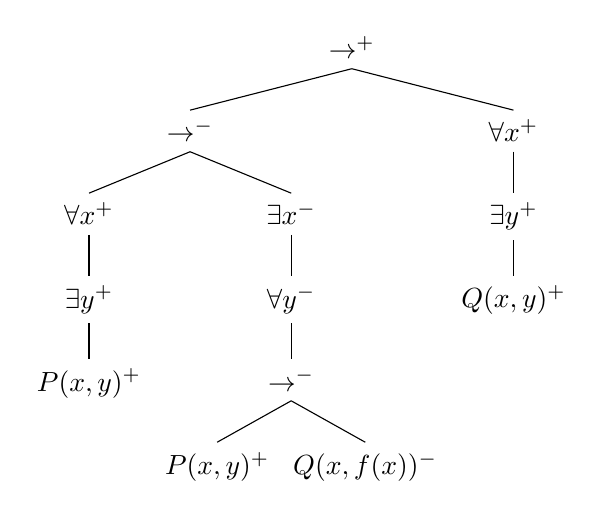
\begin{tikzpicture}
			\Tree [.$\to^+$ [.$\to^-$  [.$\forall x^+$ [.$\exists y^+$ $P(x,y)^+$ ] ] [.$\exists x^-$ [.$\forall y^-$ [.$\to^-$ $P(x,y)^+$ $Q(x,f(x))^-$ ] ] ] ]  [.$\forall x^+$  [.$\exists y^+$ $Q(x,y)^+$ ] ] ]
		\end{tikzpicture}
	\end{center}
\end{example}

We can now give sufficient conditions for when an extracted proof will always be intuitionstic:

\begin{theorem}
	Suppose in the formula tree of $\varphi$ there is no occurrence of $\to^+$ or $\forall^+$ below $\to^-$ or $\vee^+$. Then for any resolution proof $\mathcal{T}$ of $\varphi$ the extracted \Gc proof $\mathfrak{f}_2(\mathcal{T})$ is a valid \Gi proof.\\
\end{theorem}

This is however quite restrictive. Even quite simple, intuitionistically valid sequents like $$(A\to A)\to A\Rightarrow A$$ or $$(A\to B)\to C, A\to B\Rightarrow C$$ are not covered by the above theorem.\\
However by examining alternatives to rules R$\to_1$, R$\forall_1$ we can find more broadly applicable results.

\subsection{$\Pi_2$ sentences in PA}

\subsection{A refined algorithm}

Consider the calculus \Gi' obtained from \Gi by replacing R$\to_1$ and R$\forall_1$ with the rules 
\begin{center}
	\AxiomC{$A, \Gamma\Rightarrow \Delta, B$}
	\RightLabel{R$\to_2$}
	\UnaryInfC{$\Gamma\Rightarrow\Delta, A\to B$}
	\DisplayProof\hspace{2cm}
	\AxiomC{$\Gamma\Rightarrow \Delta,A[a/x]$}
	\RightLabel{R$\forall_2$}
	\UnaryInfC{$\Gamma\Rightarrow\Delta, \forall xA$}
	\DisplayProof
\end{center}
where the introductory axiom in the branch is not between atoms from $\Delta$ and $A$.

In we analyse our reasoning for theorem 5.7 under this calculus we identify for each formula precisely the atoms we may not resolve with each other.

Intuitively this corresponds to the fact that doubly negated atoms cannot resolve request.

\pagebreak


We now propose a translation procedure for formulas $\varphi$ such that $\varphi^\circ$ is provable by resolution iff $\varphi$ is valid in \Gi'. The key insight is that atoms that occur left below $\to^-$ may not be resolved with atoms that occur below only positive nodes and atoms that occur below an initial $\vee^+$ may not be resolved with atoms from the other branch of $\vee^+$:

First rename every atom $P$ to $P^0$. Rename all atoms that do not occur below a $\to^-$ to $P^1$ and all positive atoms that occurr below only positive nodes to $P^{-1}$, these atoms are not affected by any further relabelling. If a node is labelled $\vee^+$ and every node above is positive relabel all atoms $P^i$ in the left branch to $P^{i+1}$ and in the right branch to $P^{i+2}$. The thus obtained formula we call $\varphi^\circ$ and for each atom $P$ we denote the maximum $i$ such that $P^i$ occurs in $\varphi^\circ$ with $\chi_P(\varphi)$.
\begin{example}The sequent $(A\to A)\to A\Rightarrow A$ gets transformed to $(A^0\to A^0)\to A^1\Rightarrow A^1$, the sequent $(A\to \bot)\to \bot\Rightarrow A$ gets transformed to $(A^0\to \bot)\to\bot\Rightarrow A^1$.
	
\begin{theorem}
	$\{P^i\to P^0\:|\:P \text{ atom in $\varphi$}, i\leq \chi_{P}(\varphi)\}\Rightarrow \varphi^\circ$ is provable by resolution iff $\varphi$ provable in \Gi'.
\end{theorem}
	

	
	
\end{example}



\bibliographystyle{acm}
\bibliography{references}

\end{document}